\section{Solution Design}

This section will describe the solution in terms of the distributed and
concurrent parts of the system and the communication protocols that we have
designed:

\begin{itemize}
\item \textbf{Distribution -- System Architecture}:
  broad view of the system architecture
\item \textbf{Communication Protocols}:
  description of communication protocols. In this section we will expose the
  reason why certain protocols have been chosen and which properties they are
  able to guaranteed for the communication of the system
\item \textbf{Distribution -- Middleware Layer}:
  description of the middleware components and their properties. In this
  section we will explain the design choices in relation to the architectural
  properties that have been chosen for the distributed part of the system
\item \textbf{Concurrency -- Application Layer}:
  description of the application components and their properties. In this
  section we will describe why our design choices leads to a correct concurrent
  system
\item \textbf{Artificial Intelligence (AI)}:
  description of how we solved the problem of computing each agent's path
  in a distributed, multi-agent, dynamic environment.
\end{itemize}


% Distribution - System Architecture
\subsection{Distribution -- System architecture}
As we previously said, our system is a simulator whose computation spreads
across multiple nodes.

We thought it was reasonable to divide it in four subsystems.
An overall view of our architecture is depicted
in Figure \ref{fig:sd-sys-arch-overall}:

asdfasdfasdfasdfasdfasdfasdf
\begin{figure}[H]
  \centering
  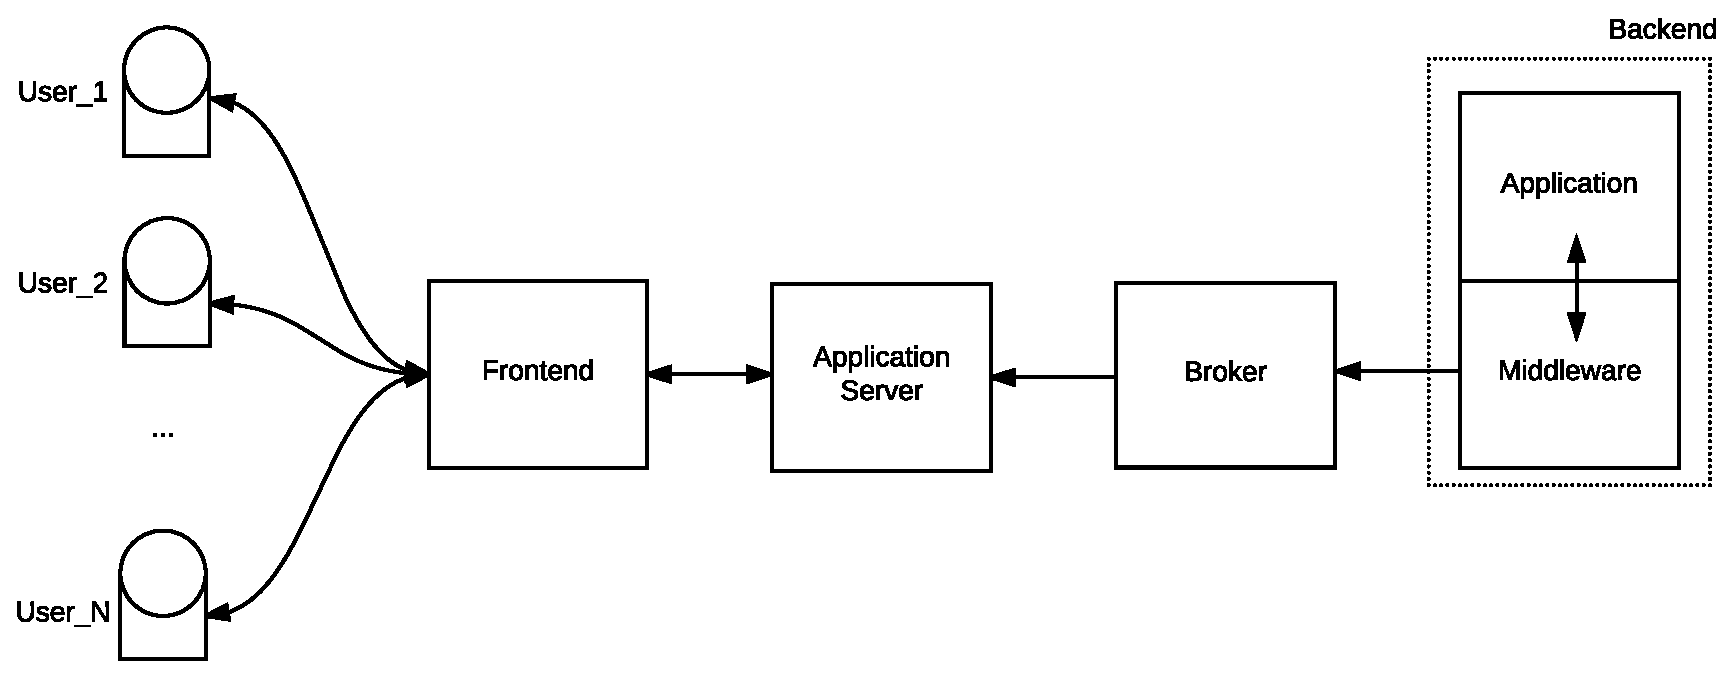
\includegraphics[scale=0.5,keepaspectratio]
    {images/solution/overall-arch.eps}
  \caption{Overall system architecture}
  \label{fig:sd-sys-arch-overall}
\end{figure}

As we can see from Figure \ref{fig:sd-sys-arch-overall}, we have:

\begin{itemize}
  \item a \textbf{Backend}, composed by the \textbf{Application} and the
    \textbf{Middleware} layers;
  \item the \textbf{Application Server}, which is responsible of handling
    information that arrives from the backend and to serve it to the frontend;
  \item a \textbf{Frontend}, which offers streaming services to end users.
\end{itemize}

Each one of these architectural macro-components can be distributed as well: we
focused our efforts on distributing the backend over multiple computation nodes
by using a \textit{2D-wrap-around topology}.
We thought this is an interesting approach to distribute our system since it
fits perfectly the way we can divide a simulated city, besides the fact this is
a topology which scales well when it comes to distribute network traffic.

In particular, we think this topology fits our needs because in our city the
most frequent application-level actions which spans over multiple nodes are
represented by a traveller which moves from a district to (obviously) an
adjacent one to continue its travel.
Therefore, if adjacent backend nodes contain adjacent districts we are able to
avoid a significant amount of unnecessary network traffic. In Figure
\ref{fig:sd-sys-arch-topology} we show a sample city, in which each district
$D_i$ is a backend node and the edges starting from each district are the links
between backend nodes:

\begin{figure}[H]
  \centering
  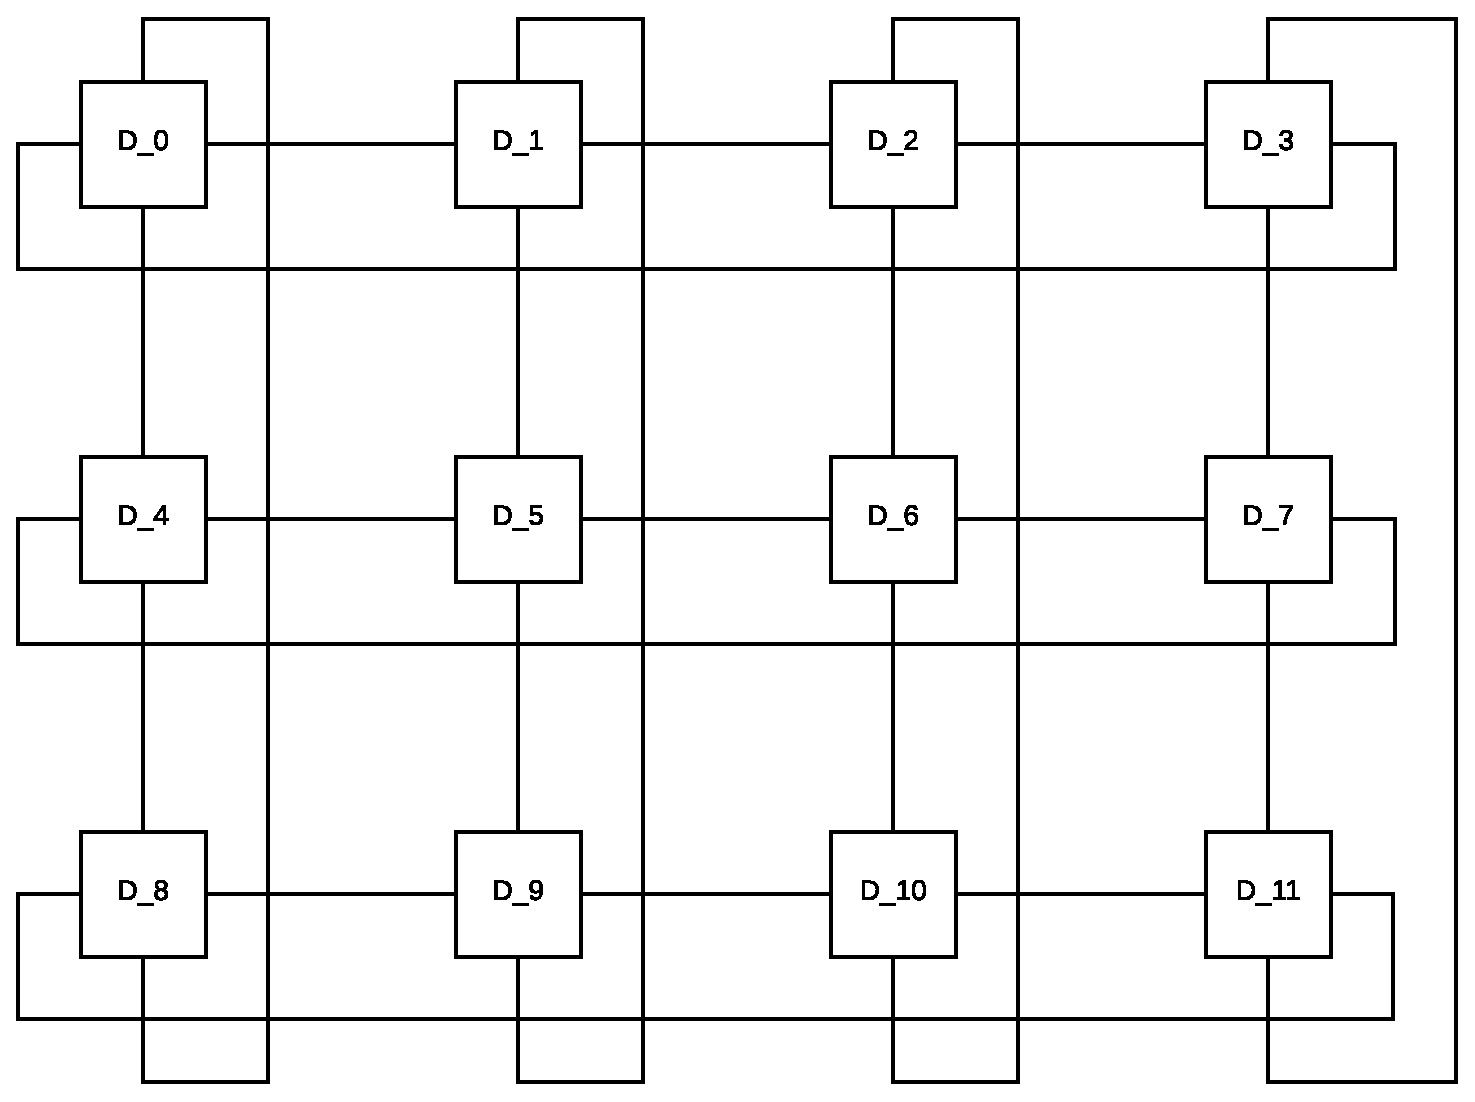
\includegraphics[scale=0.5,keepaspectratio]
    {images/solution/topology.eps}
  \caption{Sample topology for our system}
  \label{fig:sd-sys-arch-topology}
\end{figure}


% Communication Protocols subsection
\subsection{Application}
The Application is composed of two different sub-components (Figure
\ref{fig:sd-app-init}):

\begin{itemize}
  \item \textbf{Application Logic Layer}: handles the application logic
    (slightly abusing the notation, we will often refer to it simply as
    \textit{Application Layer});
  \item \textbf{Interface Layer (IL)}: provides the remote services to Application
    Layer by acting as an interface towards the underlying middleware layer.
\end{itemize}

In the next sections we will use the following terms to describe the state of a
software layer or a package:
\begin{itemize}
	\item \verb|inactive| - not even created;
	\item \verb|ready| - initialized with all the needed resources. Not yet
	allowed to execute;
	\item \verb|active| - executing;
	\item \verb|stopped| - not executing. It is waiting to terminate.
\end{itemize}

\subsubsection{Application Layer}\label{sec:sol-des-app-layer}

\input{sections/solutionDesign/architecture/app-layer/entityType.tex}



Figure \ref{fig:sd-app-backend-architecture} provides an architectural overview
of the main classes which compose the application layer.
As shown in the figure, the core packages have been named according to
Table \ref{tab:entity_type}.

\begin{figure}[H]
  \centering
  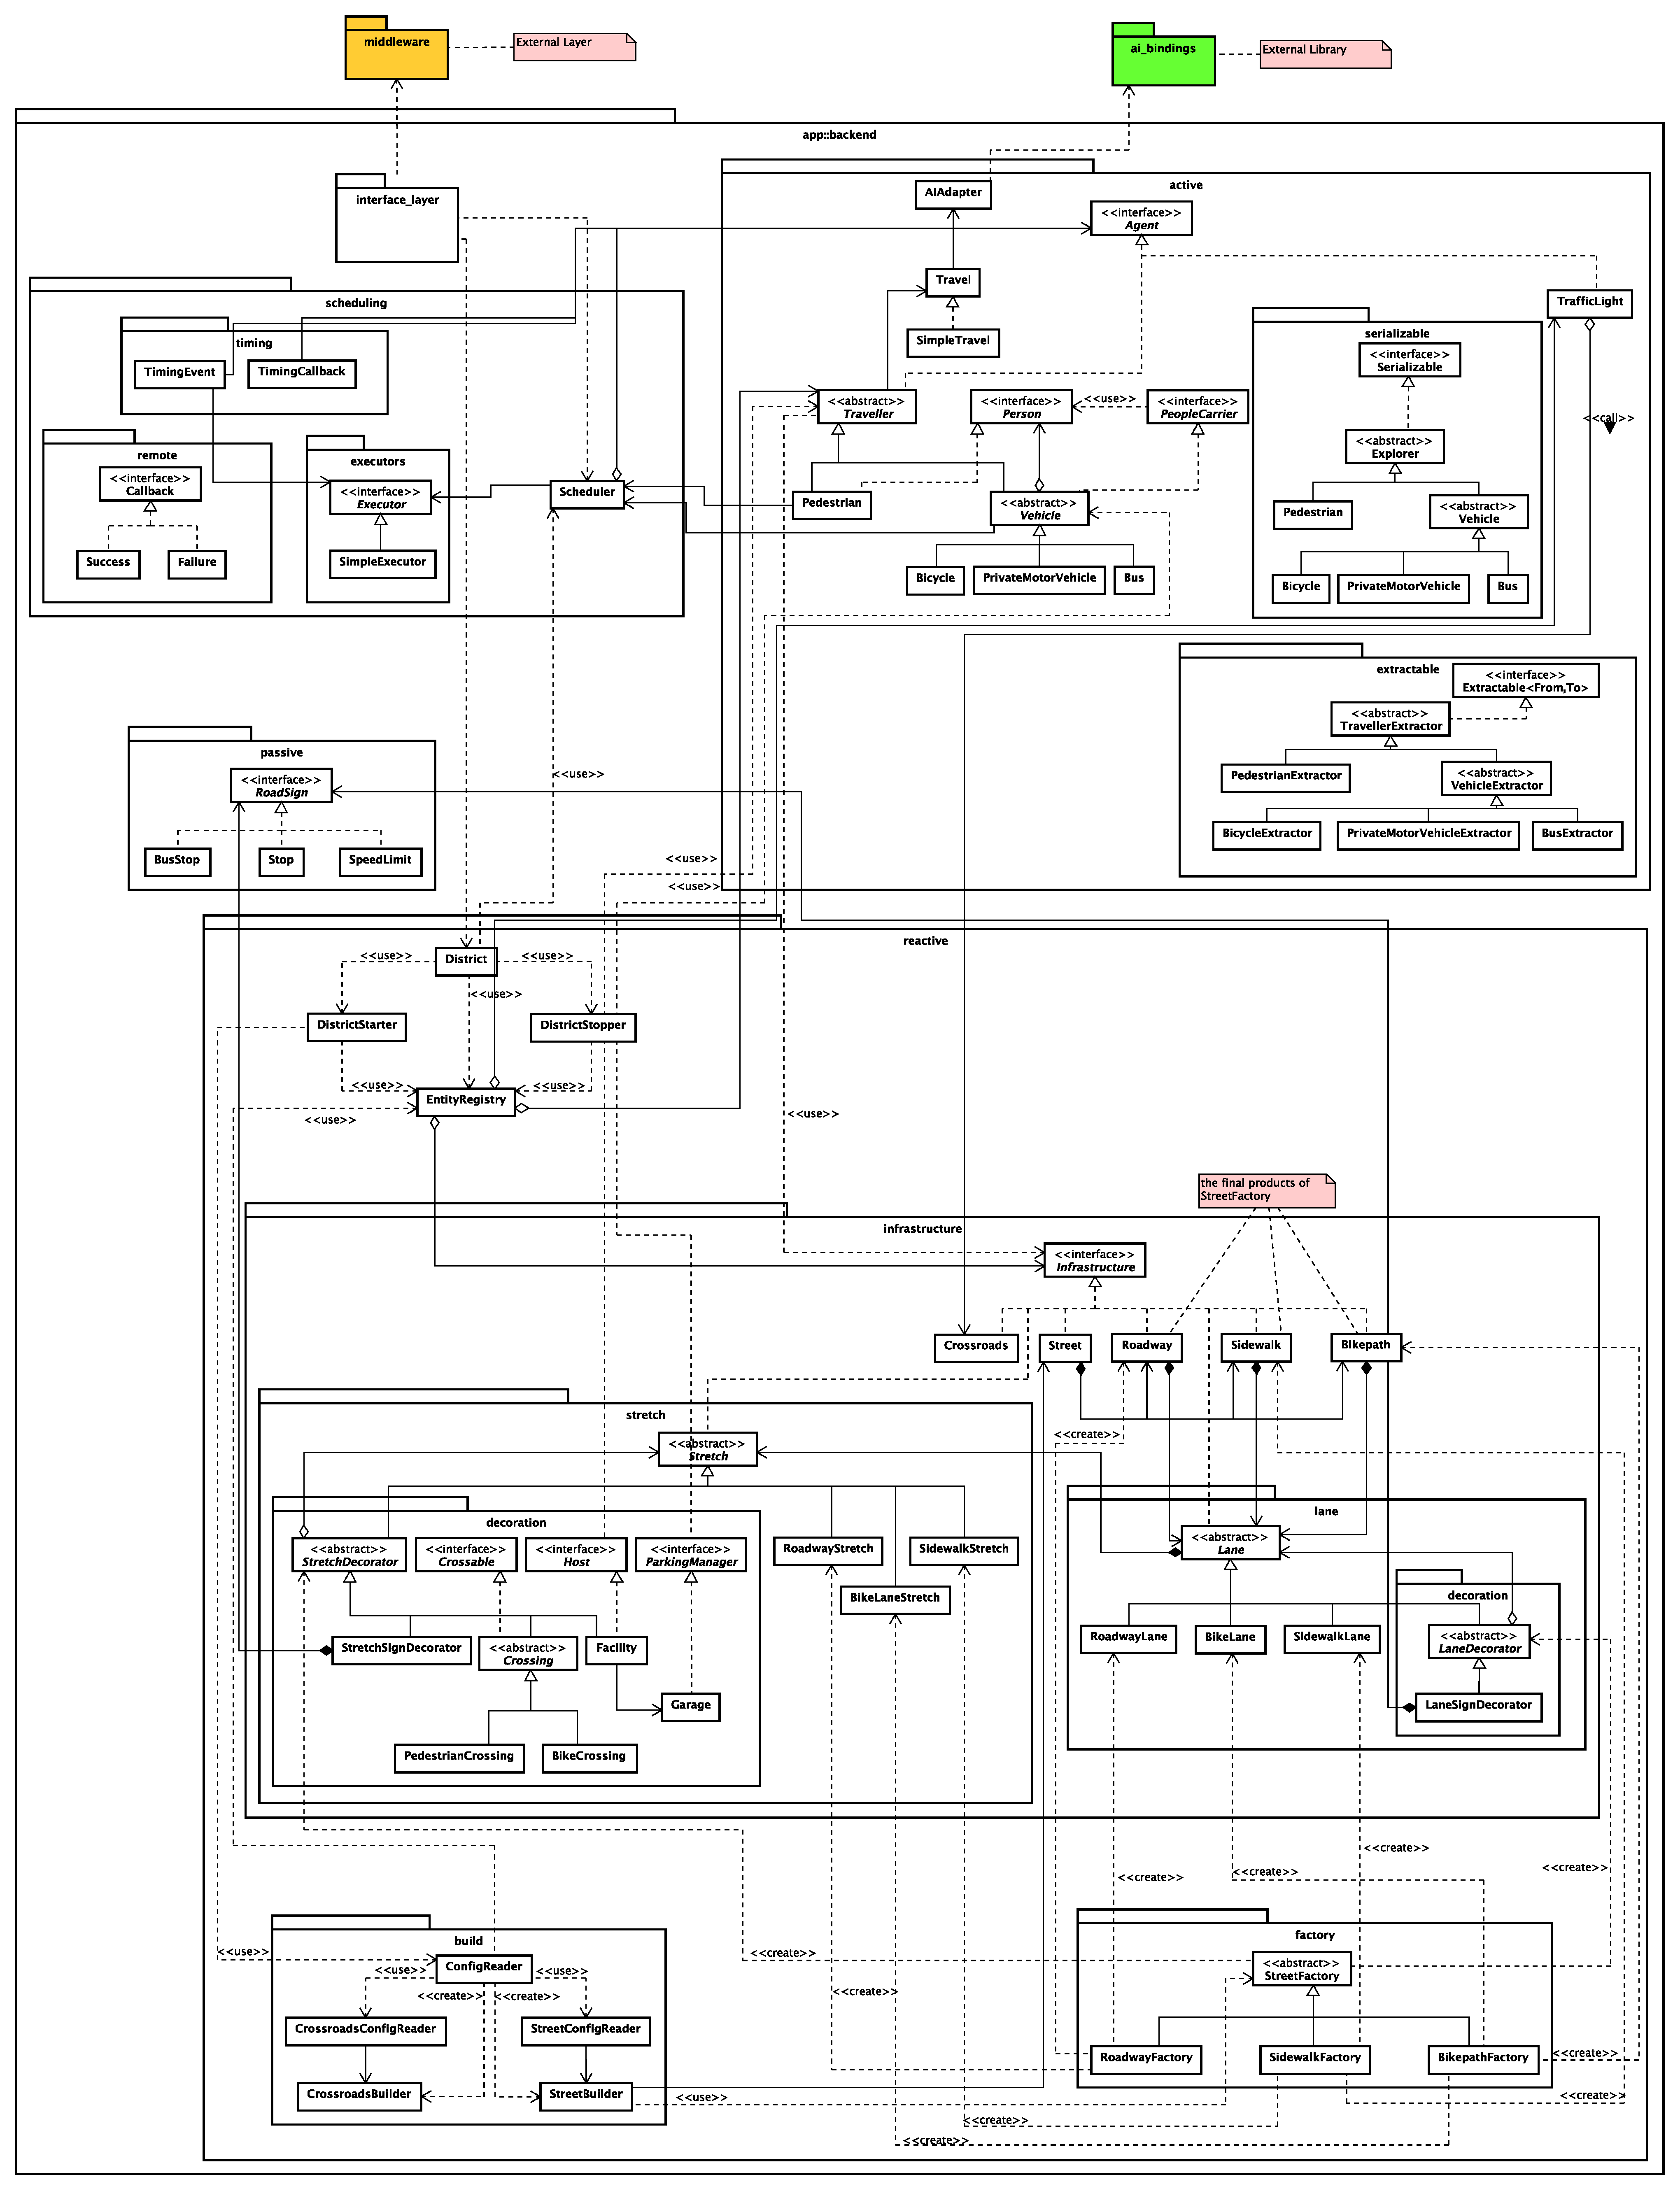
\includegraphics[width=.95\columnwidth]{images/solution/app/backend/app_backend_architecture.eps}
  \caption{Application Layer: top level design}
  \label{fig:sd-app-backend-architecture}
\end{figure}

\input{sections/solutionDesign/architecture/app-layer/active.tex}
\input{sections/solutionDesign/architecture/app-layer/reactive.tex}
\input{sections/solutionDesign/architecture/app-layer/passive.tex}
\input{sections/solutionDesign/architecture/app-layer/scheduling.tex}
\subsubsection{Artificial Intelligence (AI)}

To solve the path
problem outlined in Section \ref{sec:pa-distribution}
we have implemented a path-finder for the agents of our system.
Our AI is written in C++ but we have written the Ada bindings for it.
Thus, being able to statically link the AI to our project.

The path-finder is executed by the ACTS scheduler. In particular, a
worker runs the \verb|agent.act| procedure which contains invocations
to AI.

% The AI needs to know on which graph/infrastructure the agent
% is traveling on. Indeed, different travelers moves on different
% infrastructures. For example, a car needs to travel only on roads which are
% mostly
% separated from other city infrastructures. Thus, the AI maintains three
% search graphs, one for each infrastructure (roads, bicycle paths, sidewalks).
% In case of intersection or crossing stretches, the ids (of the stretches)
% are replicated over different graphs.


\subsubsubsection{Environment}

The first step when planning an AI consists in analyzing the task environment
to clearly understand the problem:

\begin{itemize}

\item{deterministic} -
the next state is completely defined by the previous state plus the move
performed by the agent;

\item{discrete} -
there are many state of the system, but their number is finite.
The agent acts in a discrete space and the information which he manipulates
are also discrete (e.g., costs of moves);

\item{sequential} -
the choice of the next move depends on the previous one. The agent creates
a totally ordered sequence of moves;

\item{dynamic} -
the environment change around the agent while he is computing its moves;

\item{multi-agent} -
there are several agent who act concurrently in the same virtual
environment;

\item{partially observable} -
since the system is distributed, the agent does not have access to the complete
information about the whole environment. At any time, an agent is
traveling on a
specific district which has only updated information on its state and does not
know the costs of the other districts. Also, an agent eventually needs to
compute a path which comprise several districts.
\end{itemize}

\subsubsubsection{Search algorithms}

Due to time constraints related to the path computation, we preferred to
choose a not-real-time solution. However, we recognize that a real-time solution
helped by a traffic forecast model would be more precise and interesting.
Our solution uses classical path-finding algorithms. These algorithms
belong to uninformed and informed search classes.

Our AI offers three path finding algorithms:
\begin{itemize}
  \item Greedy Search;
  \item Uniform Cost Search;
  \item A* Search.
\end{itemize}

The first one is incomplete and not optimal because of the local search which
looks only one step ahead (visiting
only the neighbors). The last two algorithm are both complete and optimal
under certain assumptions. They have been defined
to guarantee our agents to always find the best possible path with
the minimum number of visited nodes in the search graph.

\subsubsubsection{Properties}

To guarantee completeness we need to assume that each graph is a strongly
connected component. Basically, it means that there are no isolated
components. Thus, the agent knows there will always be at least a path between
the source and the destination of its plan. % its or her
\\

Furthermore, our AI considers not grid based maps: which means some common
heuristics are not applicable a priori (e.g. Manhattan distance, euclidean
distance). Also, since grid-based maps are a subset of all possible maps, we
can say that our AI is independent on the map topology.
\\

To solve the path finding problem we reason about the specific domain and its
abstractions in terms of infrastructure building blocks and travelers. We
found an admissible and consistent heuristic for A* and, more in general, other
informed algorithms. To concretely guarantee the assumptions hold for all the
graph configurations we apply the Tarjan algorithm to each of them.
\\

Tarjan automatically validates our graphs at build time by ensuring that there
is only one strong connected component for each graph. Otherwise, it reports
an error and the isolated component.
Finally, the AI is agent-independent, which means we can use it to calculate
the path of different kinds of agents: bicycles which move on bicycle lanes,
pedestrians who move on sidewalks and motor vehicles which move on roads.
Thus, each infrastructure is represented by a different infrastructure graph.
Overall, the AI manipulates three infrastructure graphs plus N costs graphs
which represent the traffic costs of a specific district.

\subsubsubsection{Heuristic}

We have approximate the dynamic component of the environment by considering
the state of the system during the simulation as a sequence of snapshots.
Thus, each snapshot can give to the path-finder the information it needs
about the city traffic.
This information is detected by a daemon process which belongs to the AI.
It uploads new generated graphs of the dynamic costs (the costs of the traffic)
in the AI graph registry. The daemon action is triggered each time a new
snapshot is generated.
\\

The traffic costs are computed as the number of agents which are on a specific
stretch when the snapshot is performed. Also, the intersections have an additional
cost given by the traffic lights which can slow down the travel of the agent.
\\

Unfortunately, the system
snapshots were not provided as planned at the beginning of the project, so
the AI computes paths always on the same infrastructure graph without
considering the traffic costs. However, its effectiveness (with traffic costs)
has been proved by running it on a city written in NodeJS for another
proof of concept simulator.

\subsubsection{Interface Layer}

Figure \ref{fig:impl-il-arch} provides an high level view of
the Interface Layer (IL) components.

\begin{figure}[H]
  \centering
  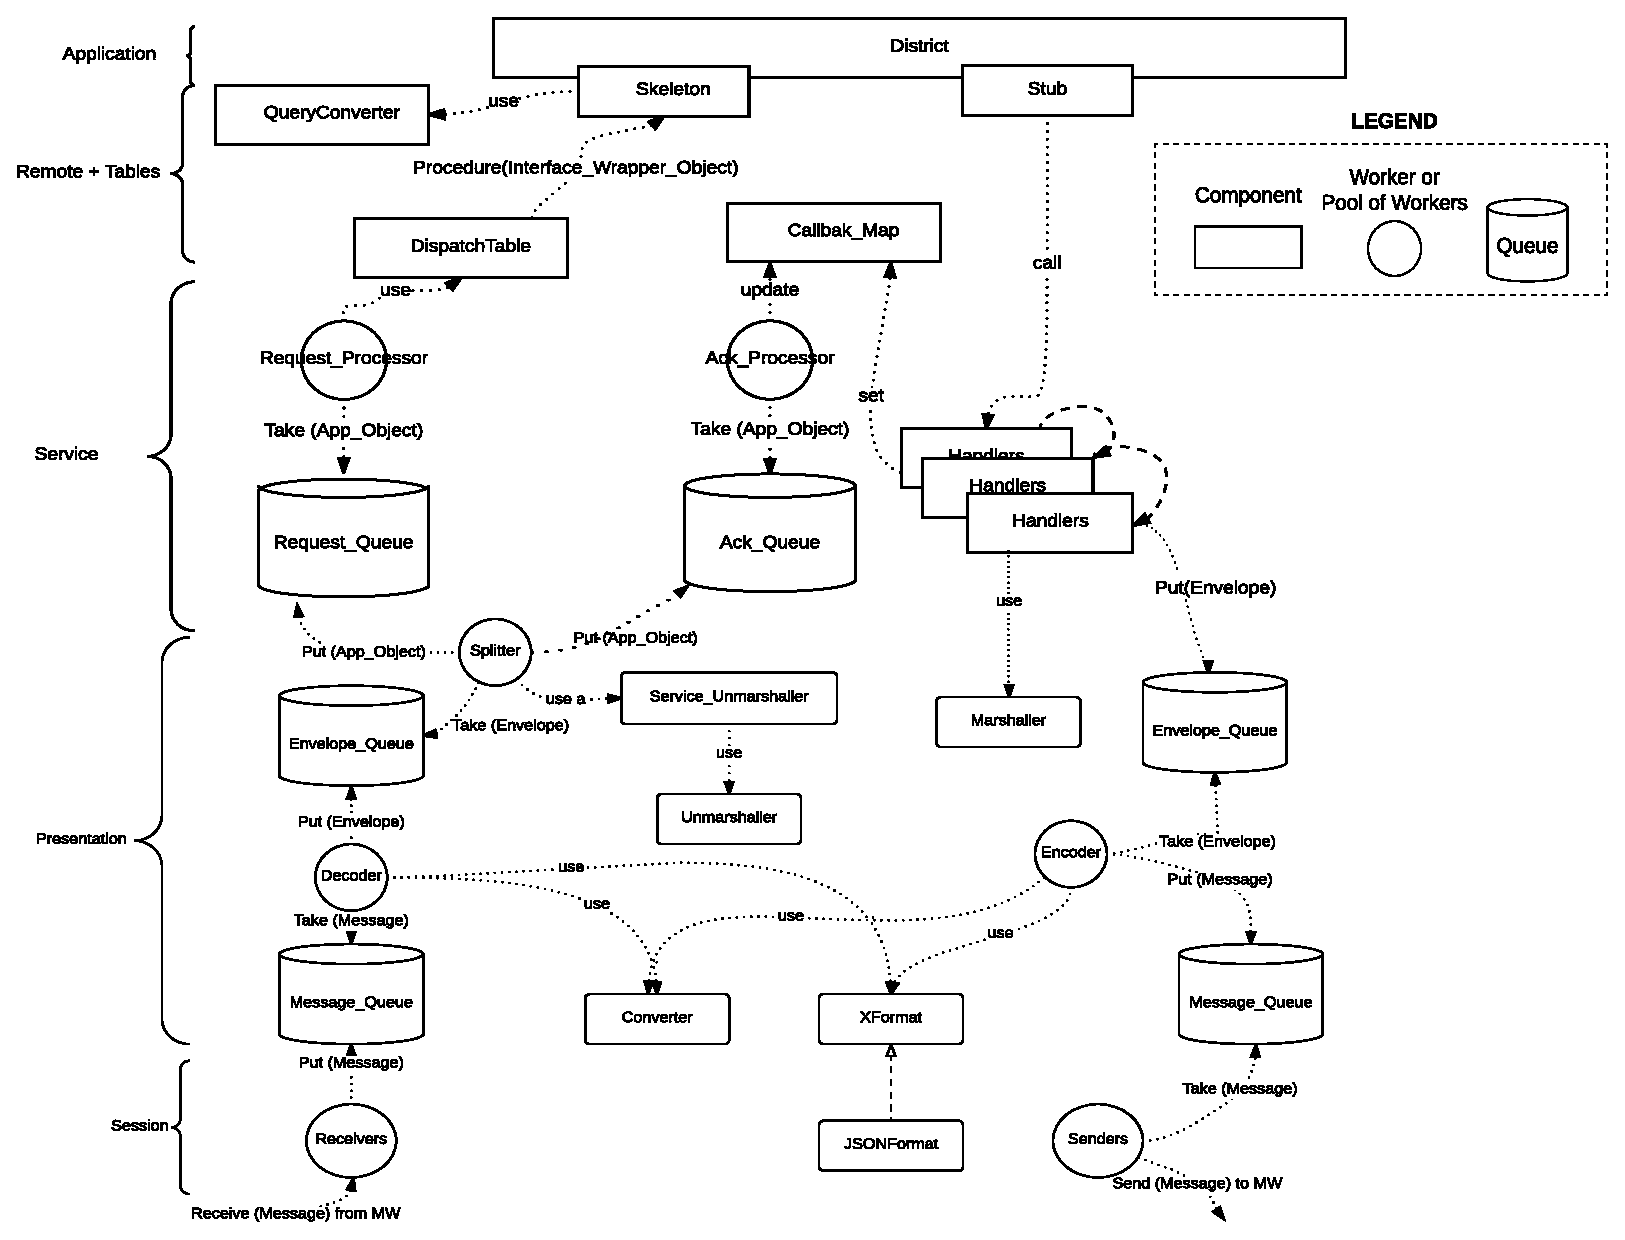
\includegraphics[width=\columnwidth]{images/solution/il.eps}
  \caption{Interface Layer architecture}
  \label{fig:impl-il-arch}
\end{figure}

IL enables the Application Layer to communicate with other applications
transparently without knowing if they are local or remote. We encapsulate the
application data as message payload while
different sublayers of IL manipulate different fields of the
message header.
This layered approach has been inspired by the TCP/IP and ISO/OSI models, in
which the layers communicate in two directions:
\begin{itemize}
	\item \textbf{horizontally:} manipulating the same fields of the header;
	\item \textbf{vertically:}  - passing the packet to the next
layer, which is charged with different responsibilities.
\end{itemize}
Also, IL is completely asynchronous because each of its sublayers has its own
thread pool. Furthermore, each thread pool is controlled by a master thread which
runs in an event loop consuming messages from its own incoming
queue. For example, the receiver can handle potentially multiple concurrent
requests by delegating each one of them to its worker threads.
After a worker has
completed the assigned task it is pushed back on the receiver's local stack,
ready to be reused.


In the following we list the sublayers which compose IL in
bottom up order:

\begin{itemize}
  \item \textbf{Session Layer:}
  handles remote connections through TCP sockets;
  \item \textbf{Presentation Layer:}
  handles messages formatting and conversions;
  \item \textbf{Service Layer:}
  converts remote requests into procedure calls
  by leveraging a skeleton object.
  Also, it offers the specular service through a stub object plus a pipeline
  of handlers. For each request, the former compose a specific pipeline
  of handlers transparently to the Application Layer.
  The handlers are used to incrementally construct the message by adding
  header fields, wrapping the data into a payload field and finally putting
  the message in the first queue which goes downwards (towards the middleware).
  \item \textbf{Remote Layer + Tables:}
  It contains the tables used
  to dispatch the remote calls and the callback map of pending requests.
  A pending request is a synchronous requests which may trigger one of
  the following behaviors:
  \begin{itemize}
  	\item retransmission on timeout;
  	\item a local retry on failure - retry on the local district with
  	the next action which could be a repetition of the last executed action;
  	\item a local clean up on success - remove the retained data from the local
  	district. The message has been successfully sent.
  \end{itemize}
  With pending request we are not reinventing a weakened version
  of TCP retransmission timers as it might seem.
  Indeed, we have concretely faced network connection errors during
  the communication
  with the middleware layer. This was caused by occasional failures or network
  problems subsequently fixed by the system itself
  (i.e., the docker swarm node).
  However,
  we preferred to give the responsibility of these synchronous messages to IL
  for two reasons:
  \begin{itemize}
  	\item it is the layer which has the highest probability of not losing them.
  	Indeed, the communication with the Application Layer happens through
  	local procedure
  	calls. Also, the TCP communication with the middleware layer could lead to
  	lose messages;
  	\item the data wrapped in the messages are important for the
  	application which can not afford to lose them. Indeed, a lost message
    could mean a missing pedestrian in the system. Thus, a failure
  	or a timeout has to trigger a reaction as soon as possible because
  	the latency introduced in the communication can lead to a significant
  	time drift for the end user (e.g., a set of travelers blocked with
  	apparently no reason). This could undermine the principle of viewing the
  	whole distributed system as one single unit.
  \end{itemize}
\end{itemize}
\subsubsection{Bootstrap}

The bootstrap process consists of two ordered and separated processes:

\begin{enumerate}
  \item \textbf{Initialization:} instantiates and configures the necessary
    resources for the application;
  \item \textbf{Activation:} starts the application.
\end{enumerate}

Clearly, the activation phase depends on initialization.
While the initialization process is automatically triggered at node creation,
this is not the case for activation, which is instead triggered by the
middleware.
Moreover, at the Application Layer level, we have to consider the dependencies
among the entity types (which are depicted in Figure
\ref{fig:sd-entity-types-deps}).

The overall bootstrap process, which mimics UNIX init \cite{online-tlsag},
is divided in two ordered parts:
\begin{enumerate}
  \item \textbf{Init:} initialize all the sublayers of each macro layer,
  following a bottom up approach (from \verb|interface_layer.session| to
  \verb|application.scheduling|).
  The initialization order is given by the fact that the upper
  layers need the services provided by the underlying layers to work
  correctly (Figure \ref{fig:sd-app-init});
  \item \textbf{Start:} IL forwards the start message sent from the
  middleware to the Application Layer.
  Therefore, this event is exclusively triggered by the middleware.
\end{enumerate}

\begin{figure}[H]
  \centering
  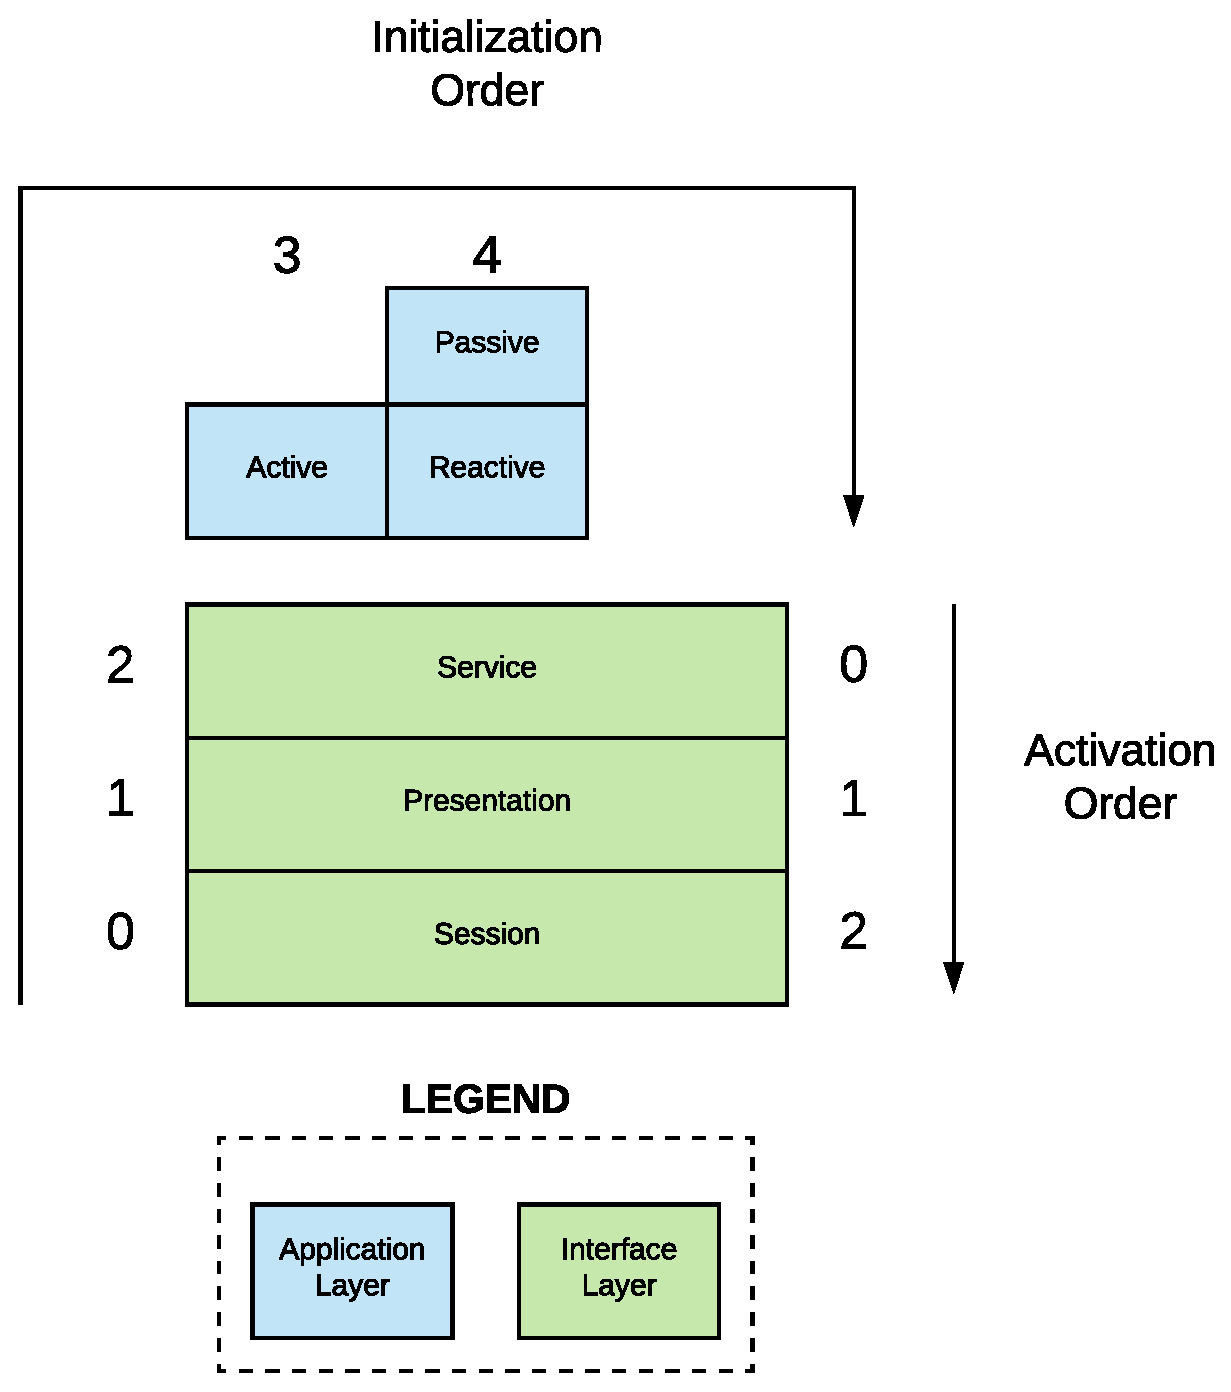
\includegraphics[scale=0.5,keepaspectratio]
    {images/solution/init_activate.eps}
  \caption{Application Bootstrap - Init}
  \label{fig:sd-app-init}
\end{figure}


\subsubsubsection{Init}

Each application node contains the \textit{Init} process,
which is the parent of all the application processes.
The execution steps of \textit{Init} are depicted in Figure
\ref{fig:sd-app-init}.
It instantiates the resources of each layer, thus making
Interface Layer and Application Layer transit from the \verb|inactive|
to the \verb|ready| state.
For example, each sublayer of Interface Layer instantiates its own pool of
LWPs\footnote{lightweight processes}.

The Application Layer initialization completes in the following order:

\begin{enumerate}
  \item \textbf{Active:} the entities which move in the city (e.g.,
    pedestrians);
  \item \textbf{Reactive:} the infrastructure of the city (e.g., streets);
\end{enumerate}

The Scheduling package, which manages the execution order for the events of the
Application Layer, does not require an initialization step. This package
will be started directly through the start message.


Since the \textit{Passive} entities are stateless and
logically belong to \textit{reactive} entities (e.g., speed limits belong to
roads), they will be instantiated along with them
(Figure \ref{fig:sd-entity-types-deps}).

When \textit{Reactive} completes its initialization, \textit{Init}
signals the Application layer completion to each sublayer of Interface Layer
in the following order:

\begin{enumerate}
  \item \textbf{Service:} provides activators and pipelines services to
    application layer;
  \item \textbf{Presentation:} provides data conversion services;
  \item \textbf{Session:} provides network connection services (e.g., senders
  and receivers).
\end{enumerate}

\textit{Init} triggers the transition of each IL sublayer state from
\verb|ready| to \verb|active|.
The activation order is extremely important to proactively avoid
message losses between remote nodes.
Indeed, at this stage, the application layer is
not able to generate or receive messages because the start message has not
been sent by the middleware. Obviously, IL is a reactive component
of the backend subystem. Thus, its \verb|active| state means
that all the workers of IL have started their event loop.
Their loop execution is triggered each time a
message arrives. Indeed, the workers are blocked on unbounded synchronized
queues which have been designed to be thread safe \cite{taft2006ada}.


The service and the presentation layer are activated before the session layer;
the latter exposes a remote communication channel through TCP
sockets.
Finally, the application is ready to communicate because both of its layers
has been activated.

Now, the Application waits the \verb|start|
message from the middleware.


A crash of the \textit{Init} process, occurring before the end of the
bootstrap, is detected by the middleware layer. The expiration
of a timeout triggers a retransmission from the middleware side.
Note that this model should also work for a bootstrap which is executed
starting
from a valid snapshot of the system, with the only difference consisting in
divergent values of the configuration file.
Indeed, for each simulation we will use a set
of configurations which is going to be different for each city.

\subsubsubsection{Start}

When \textit{Init} completes, the Application Layer is in a \verb|ready| state
while Interface Layer is in an \verb|active| state.
The first message sent by the middleware towards the Interface Layer is a
\verb|start| message which triggers the Application Layer activation.

The \verb|start| message kickoffs the scheduler, causing it to load the set
of actions declared in its configuration file. An action is a $<$\verb|agent|,
\verb|time_span|$>$ pair, i.e., the active entity \verb|agent| will act in
\verb|time_span| milliseconds.

\subsubsubsection{Termination}
When describing the shutdown of the whole system, we assumed 
the application terminates gracefully.
In this section we show the algorithm that is used to achieve this goal.

As we can see from figure \ref{fig:app-proc-tree}, the termination follows the
opposite order of the bootstrap.

\begin{enumerate}
  \item The \textit{Master} task $M$ stops active entities, e.g. pedestrians;
  \item After stopping active entities, $M$ saves their state into a file;
  \item $M$ saves into a file the state of reactive entities. 
  It is important to notice their internal state is now safetely savable, 
  since no active entities can modify it anymore;
  \item $M$ sends an \texttt{app\_shut} message to the middleware;
  \item $M$ terminates itself and the entire application consequently stops.
\end{enumerate}

The middleware layer can request the application to stop via the
\texttt{app.shutdown} call.

The last operation the \textit{Master} task does is to send a message for apprising
the middleware layer of the successful termination of the application one.
Similarly to the bootstrap phase, the middleware expects to receive this
message within a certain amount of time. 
In order to do so, when sending the message, $M$ also starts a timeout.
Wherefore if it expires before receiving a response message from the middleware layer, 
it calls again the \texttt{app.shutdown} procedure the application exposes.

\subsubsubsection{Interaction between entities}

The application contains several interactions among entities that have to be
specified in order to understand well how to approach different problems.

\paragraph{Entering a road} Moving entities enter a road by entering a stretch
that is located at the beginning of the road and that is treadable by their
specific entity type.

\paragraph{Entering a road stretch} Moving entities who want to enter a new
road stretch can do it whenever there is room for them in that stretch. In
particular, a roadway stretch can be trod for at most one vehicle at the same
time.

\paragraph{Zebra crossings} Vehicles which want to enter a road stretch that
has zebra crossings painted on it has to wait for pedestrians or bikes to free
all stretches of that particular crossing.

\paragraph{Changing roadway lane} A vehicle that is on the i-th road stretch
which wants to change lane has to check whether the (i+1)-th stretch in the
wanted direction is free.

In that case, the vehicle enters the stretch of the other lane; otherwise, if a
timeout expires before a vehicle is able to change lane, then it gives up on
it and proceeds forward to the next stretch.

\paragraph{Crossroads} Every road that is connected to a crossroads is marked
with a cardinal point (N/E/W/S). The crossroads holds all the logic necessary
for vehicles to follow the yield rules we described in
\ref{sec:pa-domain-problems}.

There could be a situation in which there is a standstill, for example when
four cars want all to go straight in a four-way crossroads. In this case, the
crossroads will make a car yield the right-of-way to another one.

Pedestrians can only walk on the corner of the crossroads, thus passing to the
adjacent piece of road (e.g. a pedestrian that is coming from the ``southern''
side of the western road can only enter the southern street on the ``western''
side).

\paragraph{Entering a building} When a moving entity is in the stretch where
there is the entrance of a building, then it may enter the building.

If the moving entity is a vehicle, it has to wait for all other entities who
are in the intermediate stretches to move away.

\paragraph{Exiting a building} When a moving entity is exiting a building, it
has to check whether there is room for her to move out.

If the entity is a vehicle, it has to yield the right-of-way to upcoming
vehicles and to wait that eventual sidewalks or bicycle path stretches in front
of the building are free too.

\paragraph{Choosing to use a vehicle} An entity $e$ who wants to leave a
building $b_e$ to a destination $d_e$ may randomly decide not to travel by
foot. She can leave only if:

\begin{itemize}
  \item the path from $b_e$ to $d_e$ does not include any destination of other
    people who are leaving from $b$ and viceversa. Otherwise, they would share
    the vehicle if there is enough room;
  \item there is an available vehicle in $b$; and
  \item the capacity of the destination building $d_e$ is greater than the sum
    of all vehicles in it and the ones which are arriving to that building.
\end{itemize}

If all these conditions are met, then:
\begin{itemize}
  \item the entity may exit the building and travel using a vehicle; and
  \item $d_e$ now ``books'' a place for the vehicle driven by $e$.
\end{itemize}

\paragraph{Waiting for a bus} A pedestrian may randomly decide to wait for a
bus if she is on a bus stop stretch.

Firstly, she checks whether the buses that stops at that stretch match (even
partially) her path. If at least one of them does, then she wait for a limited
amount of time for a bus to arrive.

If this timeout expires, then she continues travelling by foot to the next
stretch.

\paragraph{Boarding a bus} When a bus arrives at a bus stop, then a waiting
entity will board it only if:

\begin{itemize}
  \item there is enough room for her; and
  \item this bus shortens the expected route for her.
\end{itemize}

\paragraph{Getting off a bus} A person $p$ will get off a bus when it reaches
the last stop $s$ such that $s$ belongs to the route of $p$.

\paragraph{Respecting street code} Roads and crossroads will contain all the
necessary logic to make moving entities follow the street rules.

\paragraph{Performing an overtaking} This action is possible only when a
vehicle is able to change lane. It might be triggered by a timeout which
expires when it is waiting too much for entering the next straightaway stretch.

When a vehicle tries to overtake another one, it will always try to return to
the lane where it started the operation before entering the last stretch.
% look for "manovra" translation

% \paragraph{Uber} % Is it a TODO?


% Detail design
% \subsubsection{Detailed Design}

\input{sections/solutionDesign/concurrency_applicationLayer/entityType.tex}
\input{sections/solutionDesign/concurrency_applicationLayer/detail.tex}


\subsubsection{Middleware}
\subsubsubsection{Application - Middleware}
The communication protocol between application layer and middleware layer 
\paragraph{Fire and forget} 
It is a one-way message pattern (the service sends a message without expecting 
a response). Since the application and the middleware will reside on the same 
physical node we can assume that the communication is reliable, once a message 
is sent from the application layer it arrives to the middleware layer and 
viceversa. The asynchronous communication decouples (when possible) 
the computation of the application from the computation of the middleware 
and viceversa. The standard interfaces for communication 
implemented by application layer and middleware layer enables the use of 
heterogeneous technologies for each one. Defining a standard interface 
is fundamental to abstract from the underlying technologies (implementation).

\subsubsubsection{Middleware - Middleware}

The communication between the middleware layers implies the design of different 
services. Taking into account the distributed nature of the system we have 
studied specific solutions for each service, the ideas applied come from 
well known patterns used in distributed systems:
\begin{itemize}
  \item Lamport logical clocks: in a distributed system we are interested 
in the logical sequence of the events and not the wall clock time which is 
impossible to know perfectly and could lead to synchronization errors;
  \item Lamport timestamps algorithm\footnote{Leslie Lamport \textit{Time, 
clocks, and the ordering of events in a distributed system}, ACM 21, 
pp. 558-565, July 1978}: this algorithm contains the keystone 
of each distributed service which implies a form of synchronization 
between parties;
  \item Bully algorithm: this algorithm is used in the first part of the 
shutdown process. It works dynamically and implies the election of a master 
node. 
\end{itemize}

\subsubsubsection{System Boostrap}
As pointed out in Problem Analysis (\ref{sec:pa-distribution}), the system has
to start neatly. Hence, we need to design a protocol in order to accomplish 
this goal.

The protocol is represented in figure \ref{fig:sys-bootstrap-protocol}, where:

\begin{itemize}
  \item A circle is a logical node which is composed of two layers:
    \begin{itemize}
      \item \textbf{MW}:  middleware layer
      \item \textbf{APP}: application layer
  \end{itemize}
    Since the middleware has to be application-independent, it only assumes 
    that the application layer exposes an interface through which it is 
    possible to start the application neatly;
  \item \textbf{Named arrow}: it represents a message that is sent from a 
logical node through another one with the name as its payload;
  \item \textbf{Number}: it represents the progress of the logical system clock 
during the bootstrap process.
\end{itemize}

\begin{figure}[H]
  \centering
  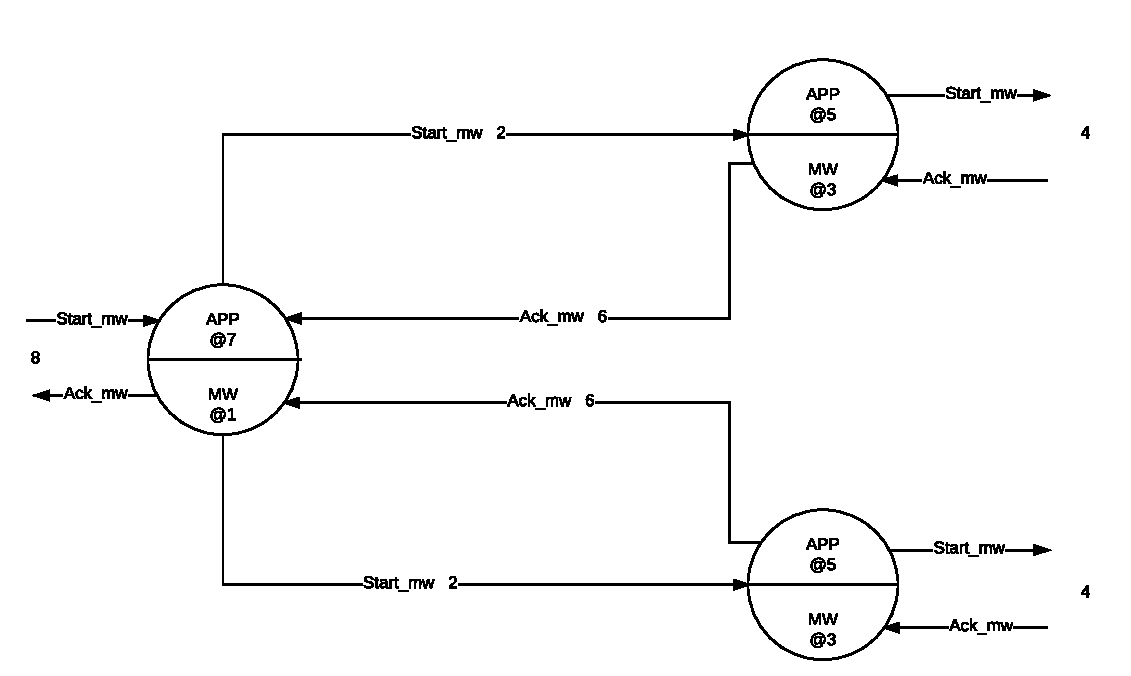
\includegraphics[width=\columnwidth]{sections/images/solution/bootstrap.pdf}
  \caption{System bootstrap protocol}
  \label{fig:sys-bootstrap-protocol}
\end{figure}

Assuming that a \texttt{Start\_mw} message arrives to a non-booted node (say
$l$) at time 0, the protocol is defined as follows:

\begin{enumerate}
  \item The leftmost node $l$ in figure \ref{fig:sys-bootstrap-protocol}
    starts its own middleware services.  
  \item $l$ sends a \texttt{Start\_mw} message to the set $S$ of all its
    neighbors. Clearly, if it was the first node in the system to receive
    \texttt{Start\_mw}, then it will be also the last node to complete the
    boot process.
  \item $l$ waits for each node in $S$ to complete the boot. $l$ waits for all
nodes in $S$ to send an \texttt{Ack\_mw} message back;
  \item The middleware MW of $l$ grants the application APP to start;
  \item $l$ then sends an \texttt{Ack\_mw} message back.
\end{enumerate}

As it can be seen in the figure, this behaviour is replicated recursively
by all nodes of the system. If a node has already been booted, then it only
sends \texttt{Ack\_mw} back.

\subsubsubsection{System Termination}
Also, the system has to shutdown neatly. Therefore we designed a protocol to
stop the entire system; please notice that this one could be seen as a
symmetric version of the System Bootstrap protocol.
% TODO: please check the sentence here above

The protocol is represented in figure \ref{fig:sys-termination-protocol}, where
the conventions are the same as the ones used in figure
\ref{fig:sys-bootstrap-protocol}.

\begin{figure}[H]
  \centering
  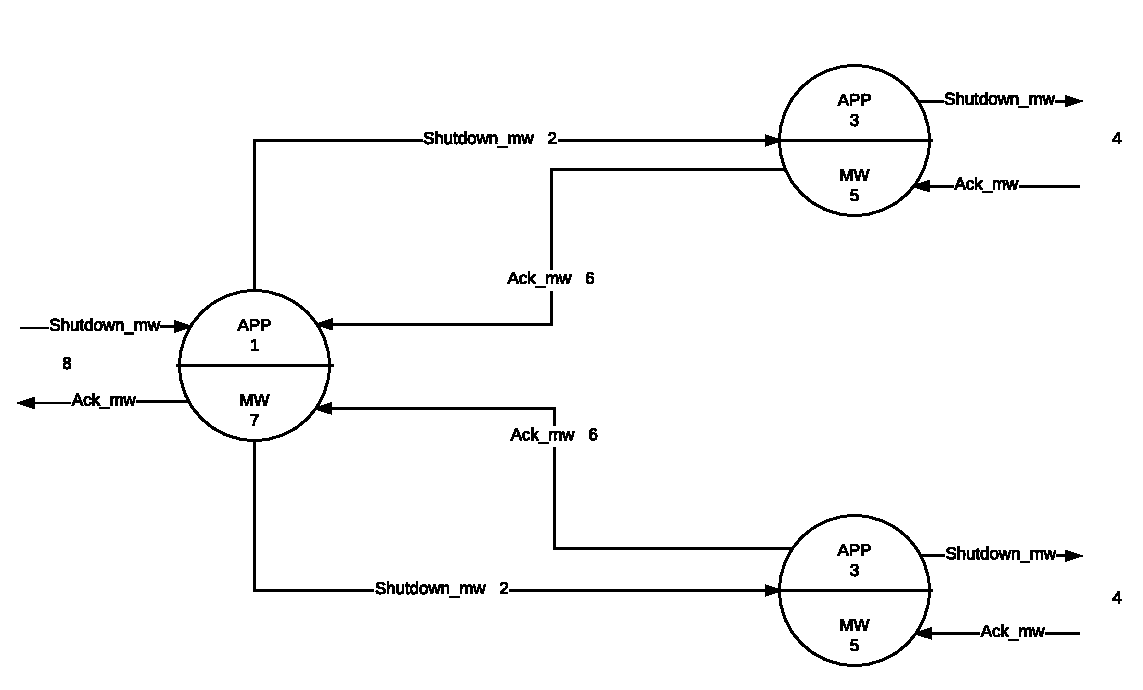
\includegraphics[width=\columnwidth]{sections/images/solution/termination.pdf}
  \caption{System termination protocol}
  \label{fig:sys-termination-protocol}
\end{figure}

Assuming that a \texttt{Shutdown\_mw} message arrives to a non-terminated node
$l$ (let it be the leftmost one in the picture) at time instant 0, the protocol
is defined as follows:

\begin{enumerate}
  \item The middleware MW of $l$ asks to terminate the application APP;
  \item $l$ sends a \texttt{Shutdown\_mw} message to the set
    $S$ of all the nodes it knows;
  \item $l$ waits for each node in $S$ to terminate, i.e. $l$ waits for all
    nodes in $S$ to send an \texttt{Ack\_mw} message back;
  \item $l$ stops its own middleware services;
  \item $l$ then sends an \texttt{Ack\_mw} message back.
\end{enumerate}

As it can be seen in the related figure, this behaviour is replicated
recursively by all nodes of the system. If a node has already terminated, then
it only sends \texttt{Ack\_mw} back.



% Distribution - Middleware Layer subsection
\subsection{Distribution - Middleware layer}
This section presents the services that make the middleware up.

Before seeing every service in detail, it is useful to have an overview to the
organization of those components.

\begin{figure}[H]
  \centering
  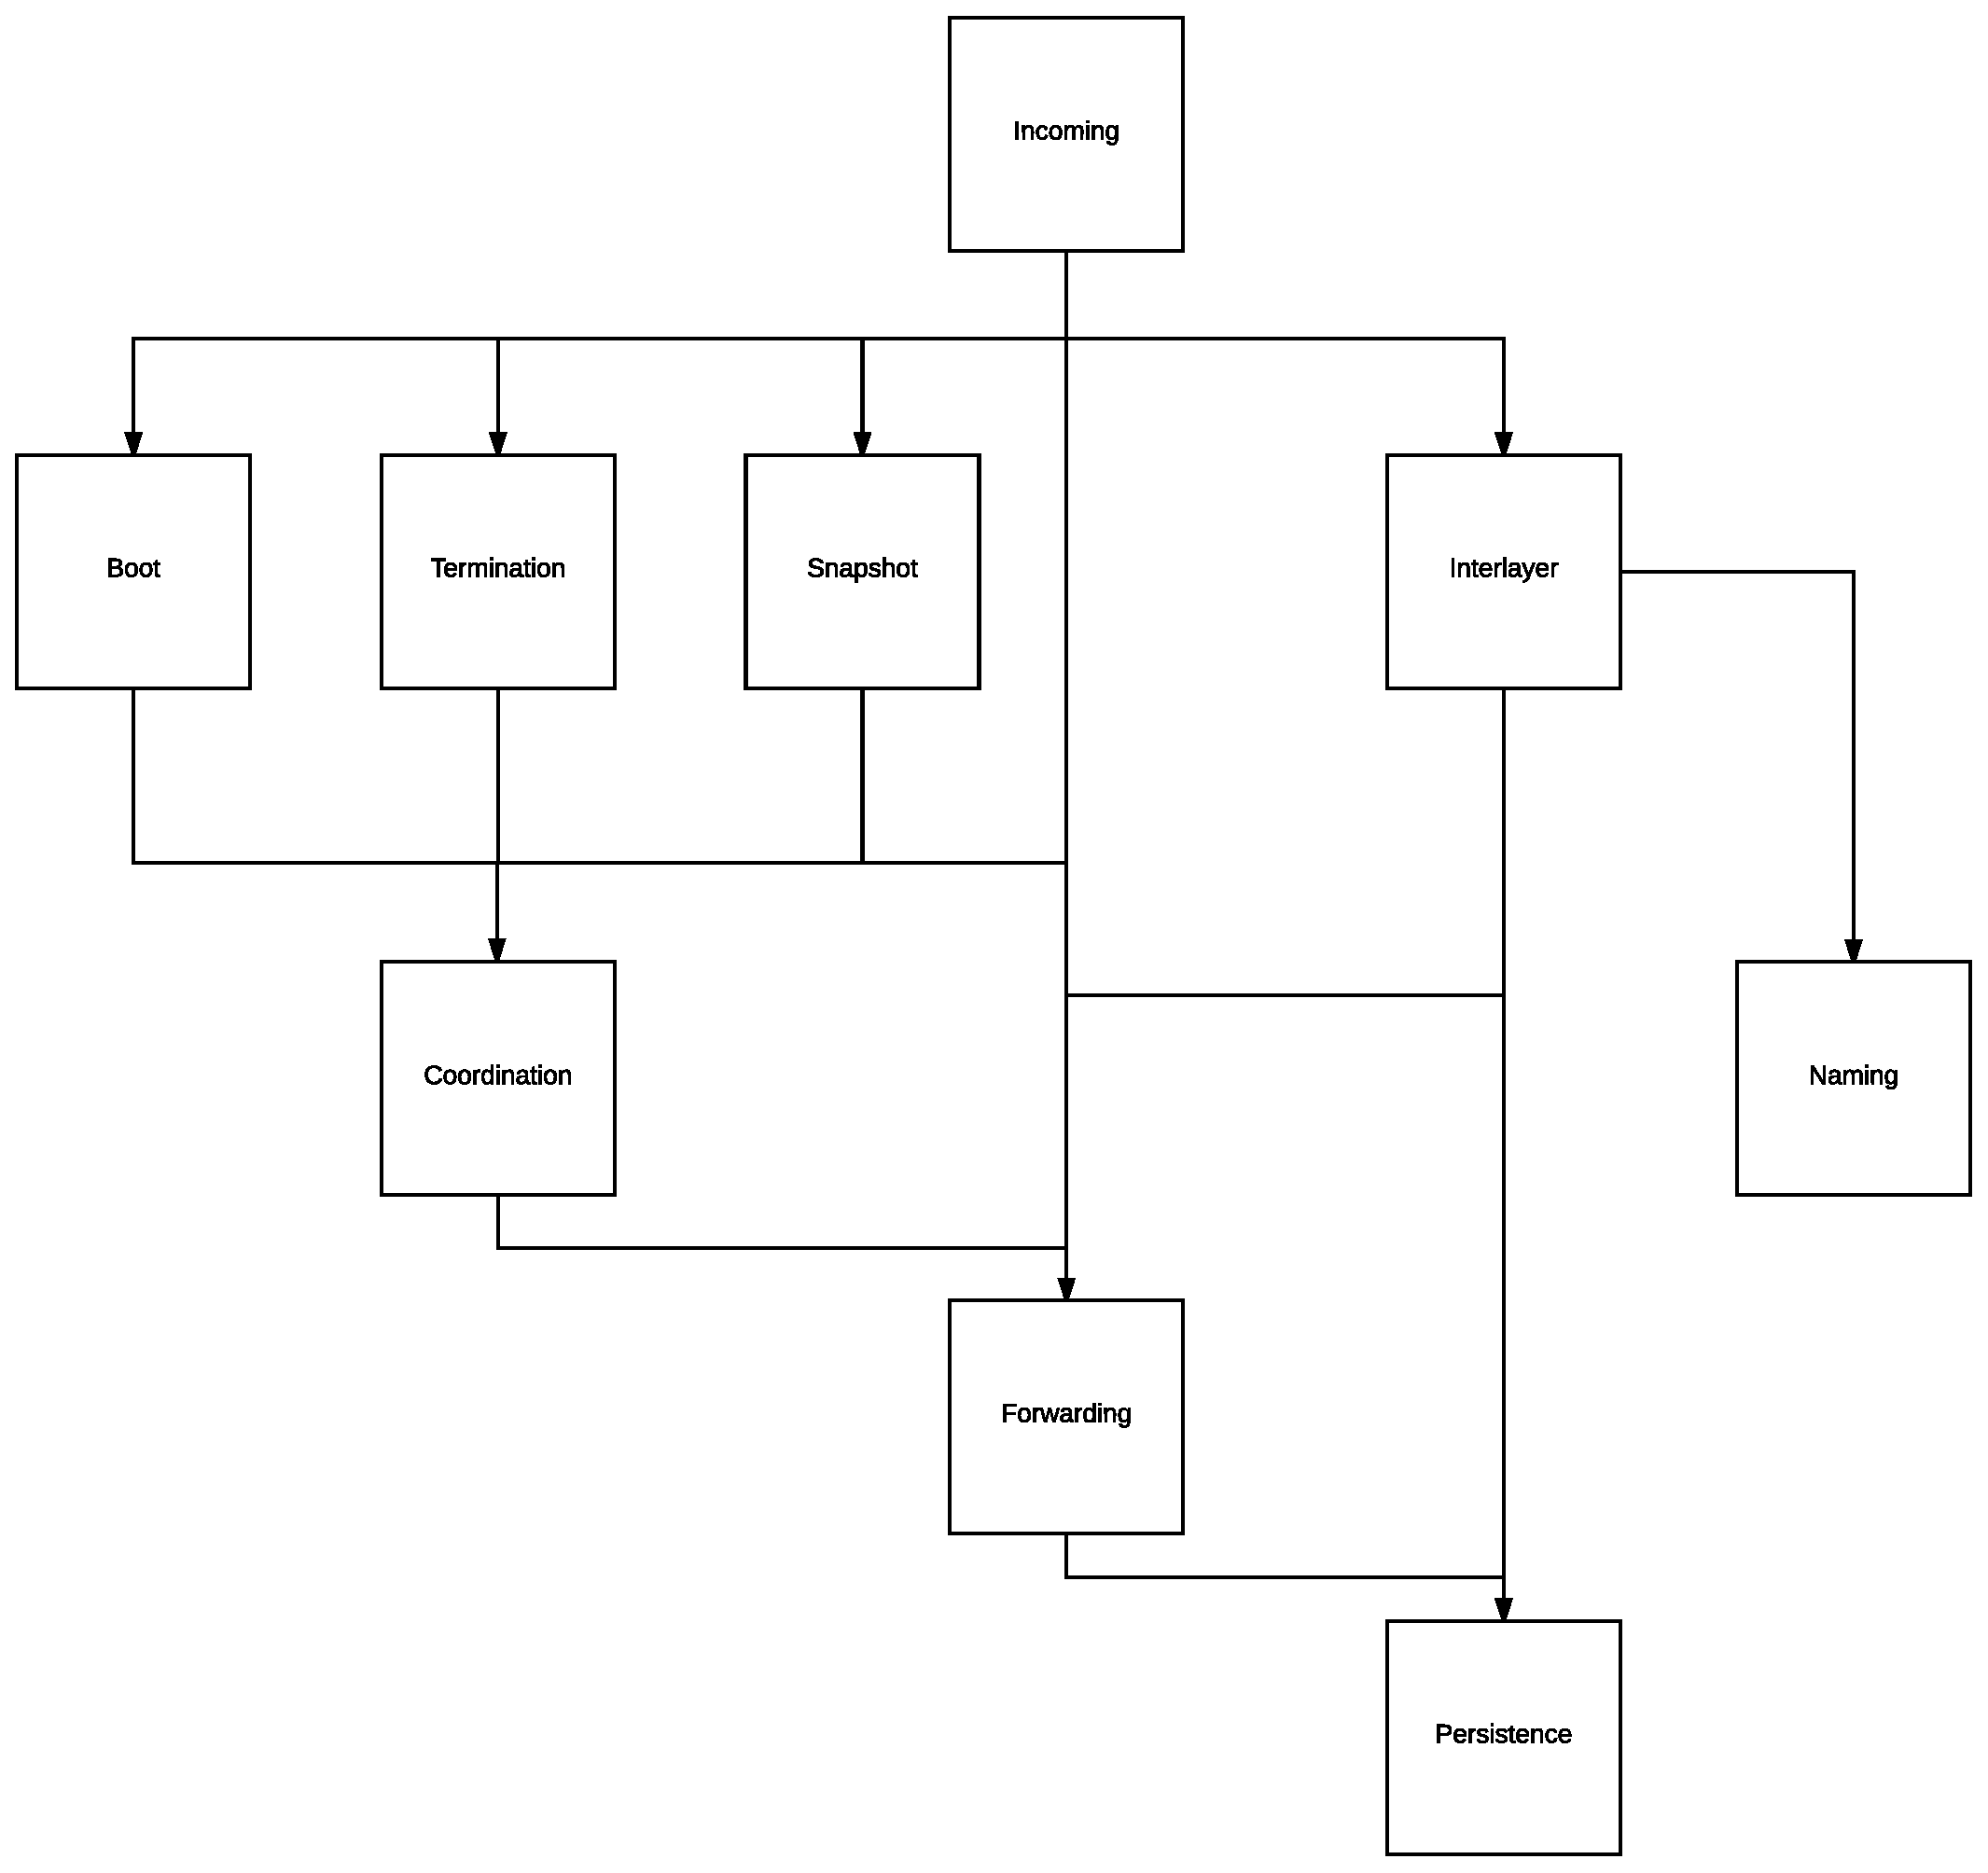
\includegraphics[width=\columnwidth]{images/solution/mw/overview.eps}
  \caption{Middleware architecture overview}
  \label{fig:mw-arch-over}
\end{figure}

\begin{itemize}
  \item \texttt{naming}: service that provides a correspondence between logic
    names and actual network addresses;
  \item \texttt{forwarding}: service that represents the abstraction through
    which it is possible to deliver messages to other middleware nodes;
  \item \texttt{interlayer}: service that represents the interface between
    the application and middleware layers;
  \item \texttt{boot}: service that is responsible to start the system neatly;
  \item \texttt{termination}: service that shut downs the node and the system
    neatly;
  \item \texttt{snapshot}: service that takes consistent views of the node and
    the system;
  \item \texttt{coordination}: service that coordinates the interaction among
    the nodes of the system.
\end{itemize}

\subsubsection{Naming service}

\subsubsection{Forwarding service}
The Forwarding service has to deliver messages to other nodes. This component
is very simple, since it just has an interface (\texttt{MQProxy}) and its
implementation, \texttt{RabbitSender}.

Basically, a \texttt{RabbitSender} takes a message as input and guarantees to
send it to the intended recipient, which could be middleware node or a
RabbitMQ pub/sub queue directed to our brokers.
\texttt{RabbitSender}s are able to make this decision by simply looking if the
messages they are handling are events or node-to-node communication. In the
first case (events), messages are propagated towards the frontend of the
application (and therefore to the brokers). In the other case, messages are
just sent to the node the sender finds in the recipient field of the message.

\subsubsection{Interlayer service}

This component is responsible of the communication that is performed among
different layers, namely the one which it belongs (the \textbf{middleware}) and
another one who uses the middleware layer, that is the \textbf{application}
layer.

We show in figure \ref{fig:mw-interlayer} the architecture of this service and
then we will show in detail each module that composes this component.

\begin{figure}[H]
  \centering
  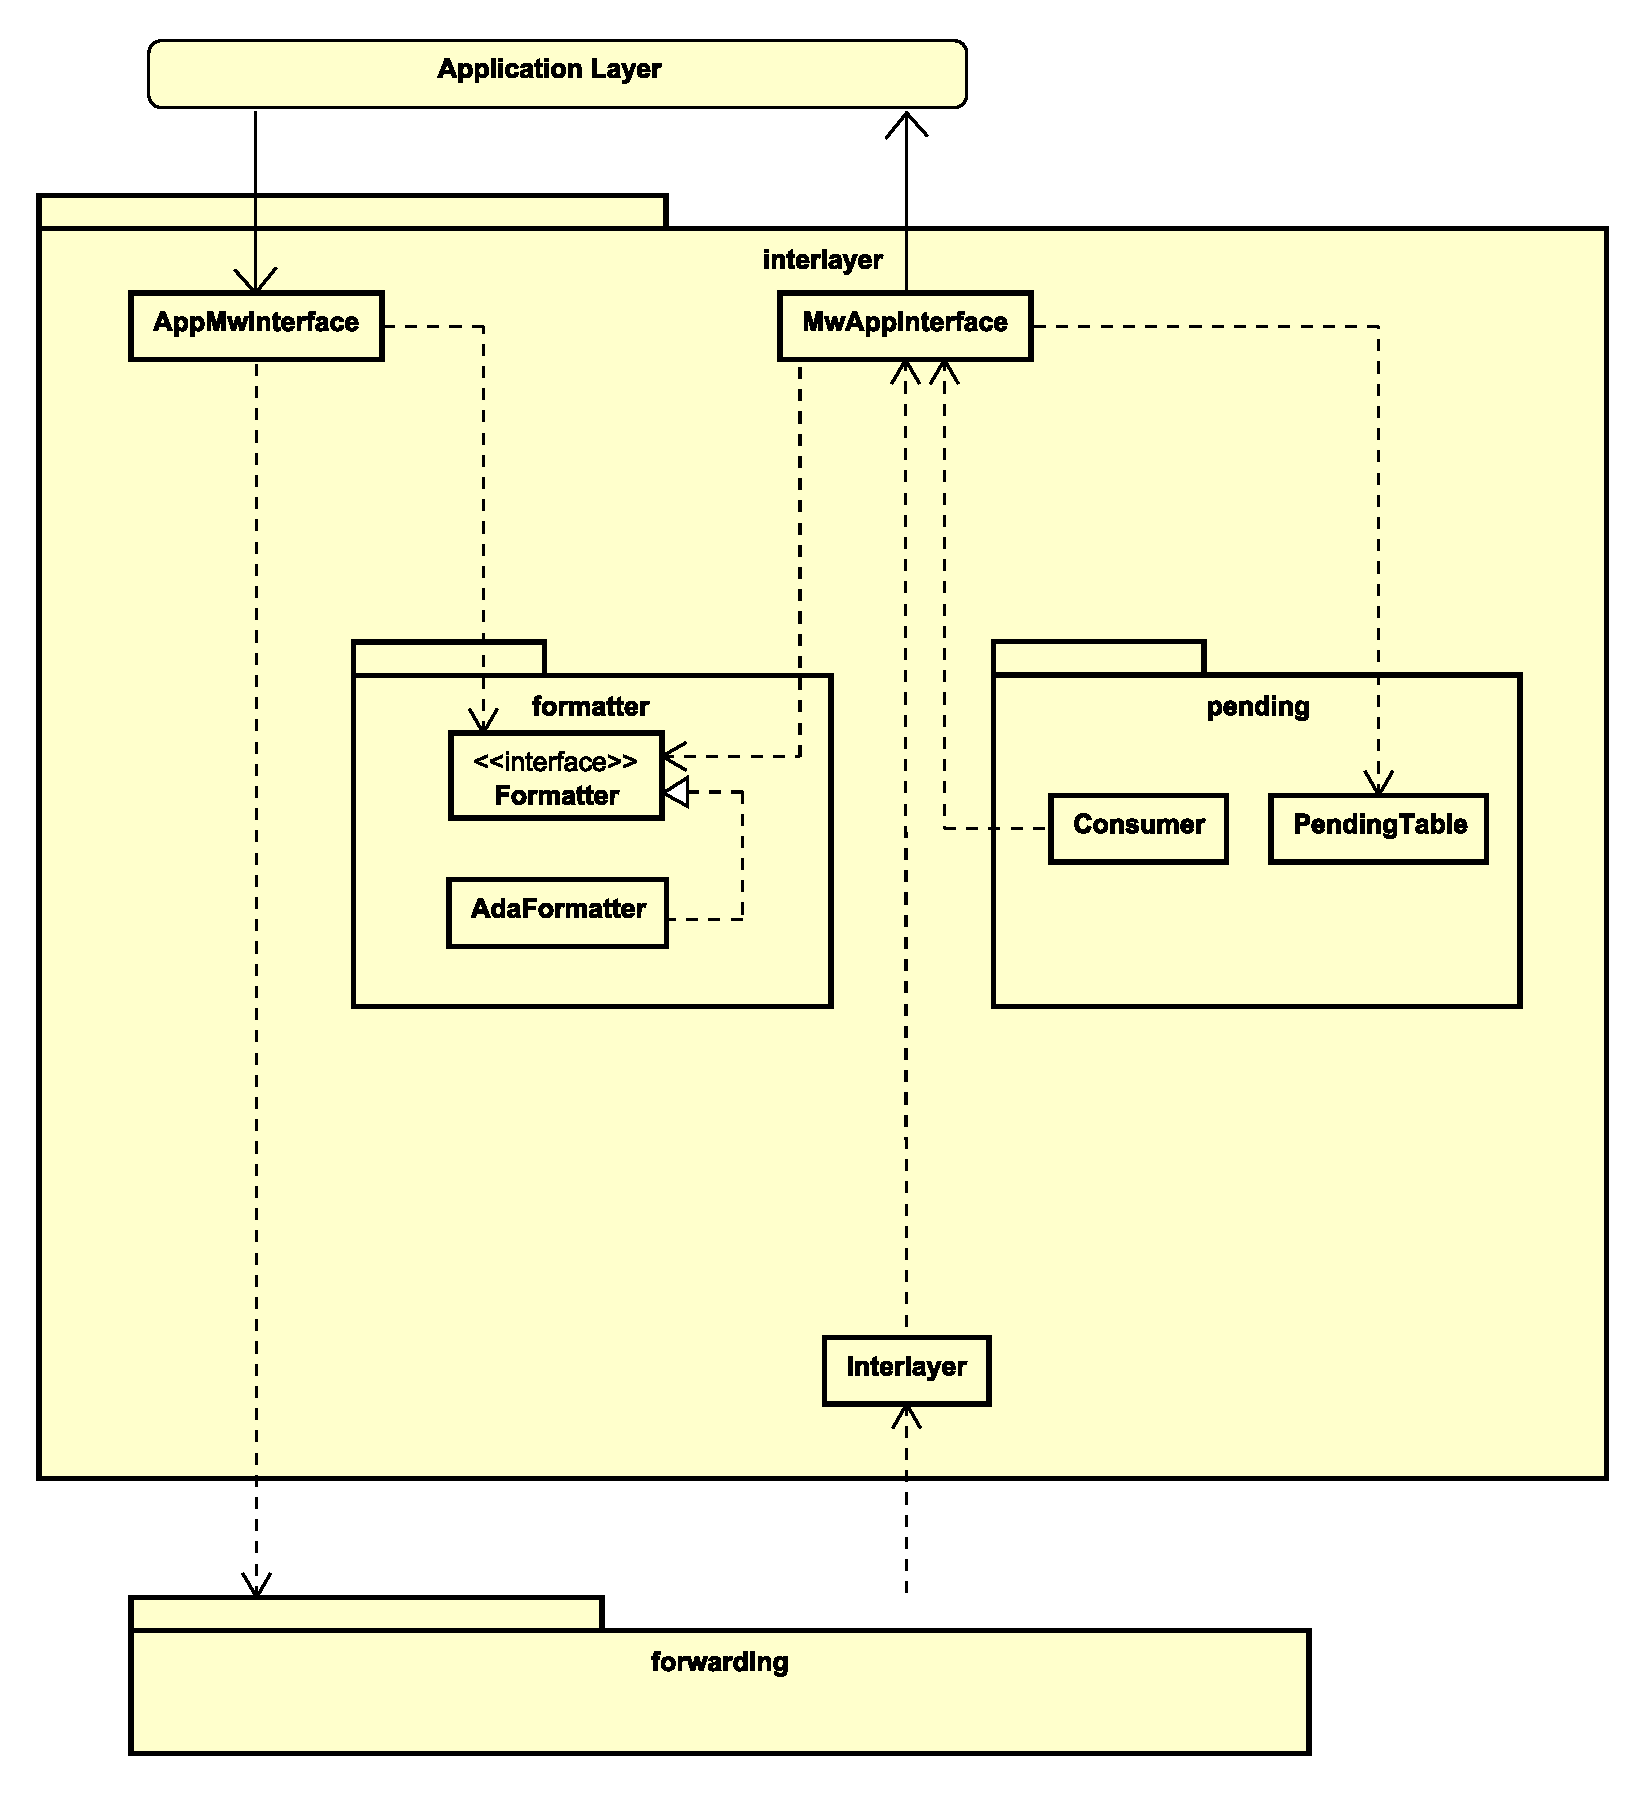
\includegraphics[width=\columnwidth]{images/solution/mw/interlayer.eps}
  \caption{Middleware's Interlayer service}
  \label{fig:mw-interlayer}
\end{figure} % TODO: needs update (Sequence usage comes from AppMwInterface)
             % TODO: how about removing AppDispatcher and Sequence?

% TODO: All class diagrams has to be added
\subsubsubsection{interlayer.Interlayer}
% TODO: Class diagram
\FloatBarrier
\begin{itemize}
  \item \textbf{Description} \\
    This module is the Fa\c cade of the Interlayer service. It is responsible
    to boot neatly and supervise all processes in Interlayer.
  \item \textbf{Attributes}
    \begin{itemize}
      \item \texttt{- sendPort: Int} \\
    TCP port messages will be directed to.
      \item \texttt{- listenPort: Int} \\
    TCP port messages will be received from.
    \end{itemize}
  \item \textbf{Operations}
  \begin{itemize}
    \item \texttt{+ start()} \\
    % TODO: check this out: Message will really be a String?
    Starts the Interlayer service.
    \item \texttt{+ handleMessage(message: String)} \\
    % TODO: check this out: Message will really be a String?
    Handles the reception of a message by ensuring it reaches the application
    layer.
  \end{itemize}
\end{itemize}

\subsubsubsection{interlayer.MwAppInterface}
% TODO: Class diagram
\FloatBarrier
\begin{itemize}
  \item \textbf{Description} \\
    Process that is responsible to deliver messages to the application layer.
  \item \textbf{Attributes}
    \begin{itemize}
      \item \texttt{- sendPort: Int} \\
    TCP port messages will be directed to.
      \item \texttt{- sendHost: String} \\
    Address messages will be directed to.
    \end{itemize}
  \item \textbf{Operations}
  \begin{itemize}
    \item \texttt{+ startLink(port: Int)} \\
    Starts the process and set \texttt{sendPort} to the value \texttt{port}.
    \item \texttt{+ toApplication(message: String)} \\
    % TODO: check this out: Message will really be a String?
    Sends a message to the application with reliable delivery.
    \item \texttt{+ send(message: String)} \\
    % TODO: check this out: Message will really be a String?
    Sends a message to the application with unreliable delivery.
  \end{itemize}
\end{itemize}

\subsubsubsection{interlayer.AppMwInterface}
% TODO: Class diagram
\FloatBarrier
\begin{itemize}
  \item \textbf{Description} \\
    Process that is responsible to receive messages from the application layer.
  \item \textbf{Attributes}
    \begin{itemize}
      \item \texttt{- listenPort: Int} \\
    TCP port messages will be received from.
    \end{itemize}
  \item \textbf{Operations}
  \begin{itemize}
    \item \texttt{+ start(port: Int)} \\
    Starts a server, setting \texttt{listenPort} to the value \texttt{port}.
    \item \texttt{- loopAcceptor(srv: PID)} \\
    Loops accepting requests as the server \texttt{srv}.
    \item \texttt{- serve(client: PID)} \\
    Handles the stream coming from the TCP connection of \texttt{client} by
    forwarding data towards to the Forwarding service.
  \end{itemize}
\end{itemize}

\subsubsubsection{interlayer.formatter.Formatter}
% TODO: Class diagram
\FloatBarrier
\begin{itemize}
  \item \textbf{Description} \\
    Interface for modules that translates messages to Elixir format from and
    to a (possibly) different one.
  \item \textbf{Operations}
  \begin{itemize}
    \item \texttt{+ format(msg: String)} \\
    Translates \texttt{msg} to the target format.
    \item \texttt{+ parse(msg: String)} \\
    Translates \texttt{msg} from the target format.
  \end{itemize}
\end{itemize}

\subsubsubsection{interlayer.formatter.AdaFormatter}
% TODO: Class diagram
\FloatBarrier
\begin{itemize}
  \item \textbf{Description} \\
    Module that implements the \texttt{interlayer.formatter.Formatter}
    interface for messages coming from an Ada application.
  \item \textbf{Attributes}
  \item \textbf{Operations}
  \begin{itemize}
    \item \texttt{+ format(data: String)} \\
    Format a message so that it can be received from an Ada application.
    \item \texttt{+ parse(data: String)} \\
    Parse a message that arrives from an Ada application.
  \end{itemize}
\end{itemize}

\subsubsubsection{interlayer.pending.PendingTable}
% TODO: Class diagram
\FloatBarrier
\begin{itemize}
  \item \textbf{Description} \\
    Process that keeps track of the messages that have not been sent yet to
    the application layer.
  \item \textbf{Attributes}
    \begin{itemize}
      \item \texttt{- pendingTable: Set<String>} \\
    Data structure in which pending messages are stored.
    \end{itemize}
  \item \textbf{Operations}
  \begin{itemize}
    \item \texttt{+ startLink()} \\
    Starts PendingTable process and retrieves pending messages from last
    execution (if there are some). \\
    Also starts an \texttt{interlayer.pending.Consumer}.
    \item \texttt{+ getnext()} \\
    If there are some pending messages, returns the first of them that has to
    be sent.
    \item \texttt{+ store(message: String)} \\
    Stores a message in the pending table.
    \item \texttt{+ remove(message: String)} \\
    Removes a message from the pending table.
  \end{itemize}
\end{itemize}

\subsubsubsection{interlayer.pending.Consumer}
% TODO: Class diagram
\FloatBarrier
\begin{itemize}
  \item \textbf{Description} \\
    Daemon worker that sequentially takes message from the pending table and
    tries to send them to the application layer.
  \item \textbf{Attributes}
  \item \textbf{Operations}
  \begin{itemize}
    \item \texttt{+ waitToConsume()} \\
    Waits for new messages to be available to be sent to the application layer.
  \end{itemize}
\end{itemize}

\subsubsection{Boot service}\label{sec:mw-boot-descr}

The Boot service is responsible of starting the system in a graceful fashion.
It does so by dividing the start phase into two subphases, namely the
\textbf{initialization} and the \textbf{boot} phase.

Initially, this service is in a \texttt{uninitialized} state, which means the
node has received neither a marker from a neighbor node to start the
initialization phase nor it has been acknowledged by the application layer that
its initialization is finished.

If the application layer tells the middleware that it's initialized, then the
Boot service will become \texttt{initialized}. If instead an initialization
marker arrives from a neighbor, the Boot service will stay in the
\texttt{uninitialized} state, waiting for the application layer to tell it's
initialized.
If the middleware receives another marker after having received the first one,
then it will reply immediately as it had finished its initalization phase.
Finally, when the Boot service has received all the initialization markers from
its neighbors and has been acknowledged by the application layer that it is
initialized, it will enter the \texttt{booting} state (and the \textbf{boot}
phase).

In the second phase this service waits for the boot marker (a middleware-layer
message which starts the boot of the system) to arrive. When it does, the Boot
service forwards the marker to all its neighbor and wait for all of them to
reply (i.e, for them to be booted).
When all the neighbors are booted, the application layer gets booted as
well and the Boot service sends a boot marker back.

The whole process is depicted in Figure \ref{fig:mw-boot}.

\begin{figure}[H]
  \centering
  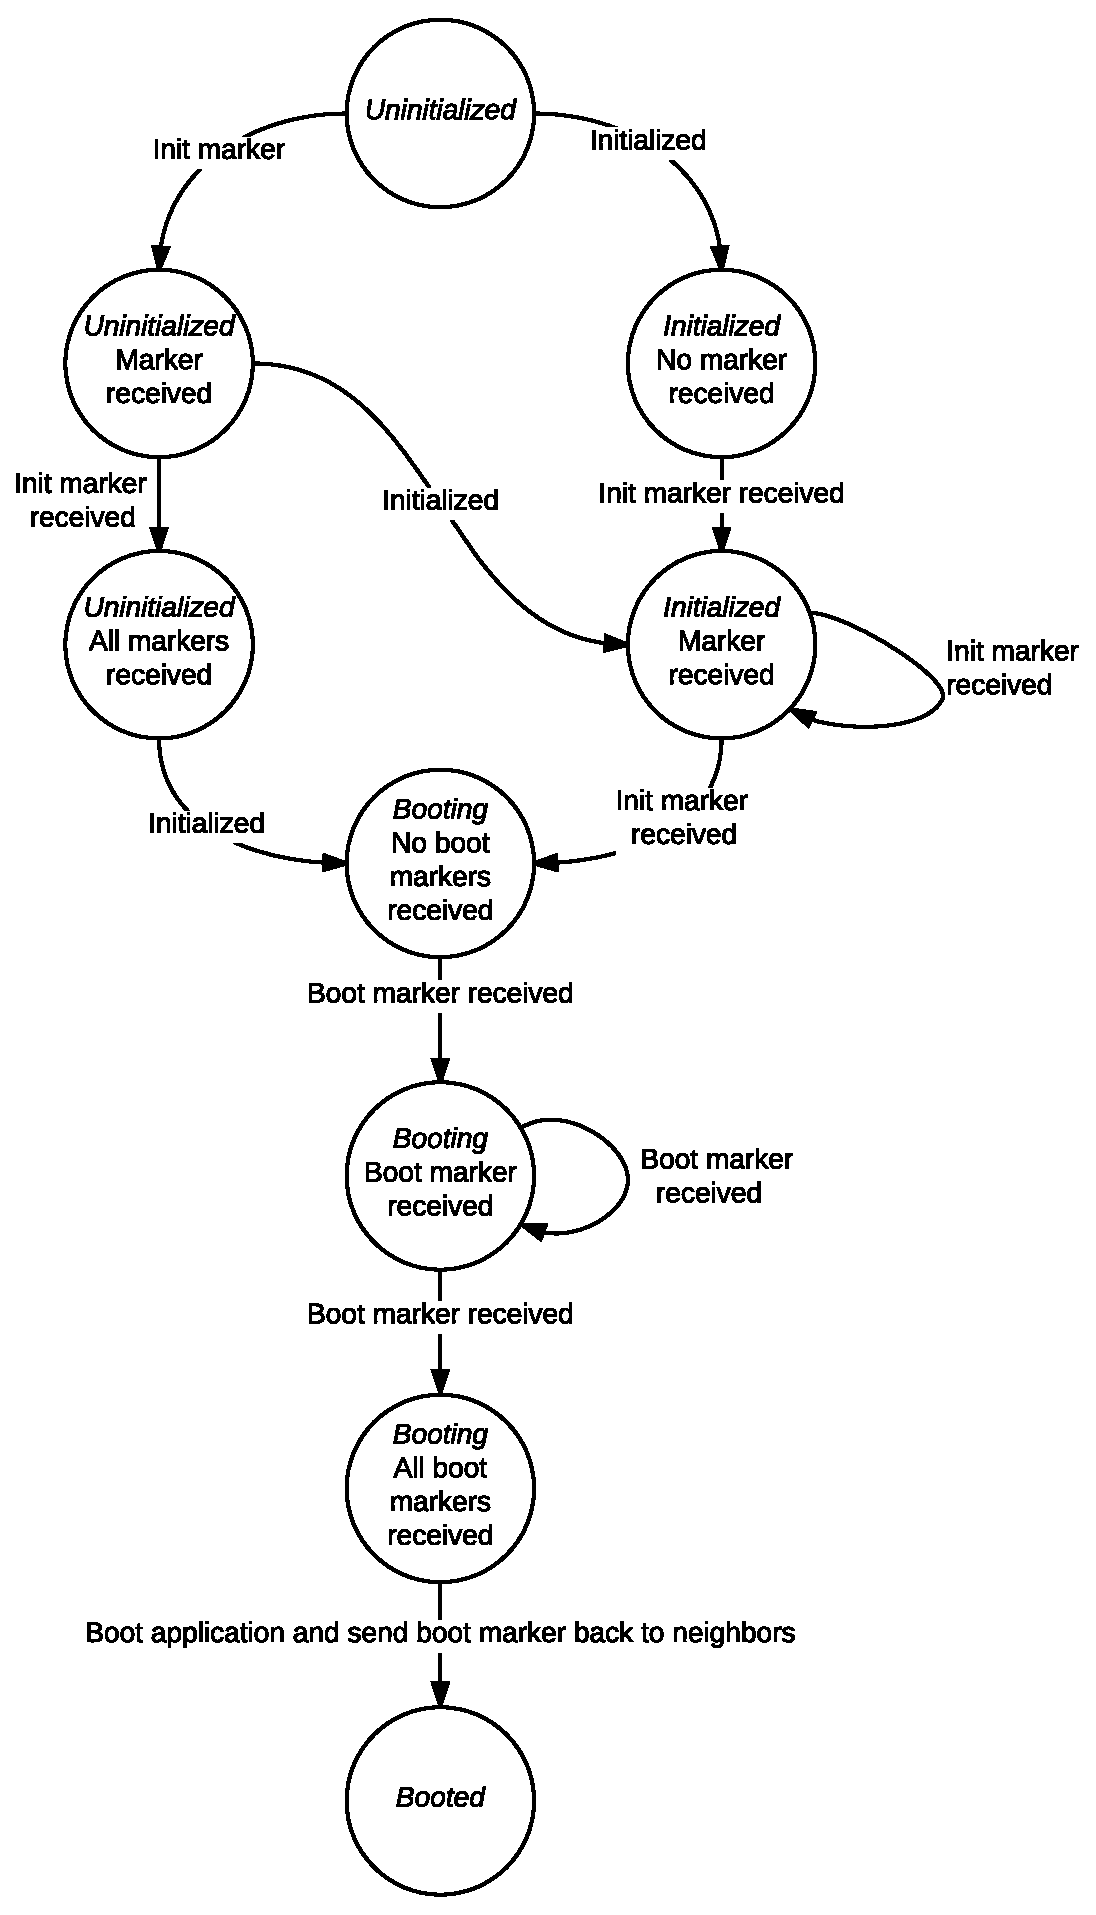
\includegraphics[width=.8\columnwidth]{images/solution/mw/boot.eps}
  \caption{Boot service: activity diagram}
  \label{fig:mw-boot}
\end{figure}

\subsubsection{Termination service}

\subsubsection{Snapshot service}

\subsubsection{Coordination service}

This component is responsible of the supervising the life-cycle of an
application run on our middleware, so our backend is able to operate
cohesively.

There are just two architectural units which compose this service:

\begin{enumerate}
\item a \texttt{Coordinator} initiates the boot process when requested and the
  termination process when the time limit for the application elapses;
\item \texttt{Monitor}s supervise the status of some services. In
  particular, we instantiated two monitor processes, one for the boot process
  and another one for the termination process. If a process $X$ does not end
  within a pre-configured time limit (we arbitrarily set 15 seconds for this
  parameter) after being started, the monitor issues again a request to
  perform $X$.
\end{enumerate}



% Concurrency - Application Layer subsection
\subsection{Concurrency - Application Layer}
This section presents the concurrent entities forming the application layer of the system.
\paragraph{Types of entities}
Three types of entities have been identified
\begin{itemize}
  \item \textit{Active}: entity capable to start an action by itself if provided 
the necessary computational resources;
  \item \textit{Reactive}: entity that only reacts to provided inputs, 
not capable to start an action by itself;
  \item \textit{Passive}: a stateless entity.
\end{itemize}
\begin{table}[H]
\centering
\begin{tabular}{|l|l|}
\hline
\rowcolor{BlueGreen}
Type     & Entities                                 \\ \hline
Active   & pedestrian, car, bus, bicycle, semaphore \\ \hline
Reactive & road, crossroads, house                   \\ \hline
Passive  & road signs                               \\ \hline
\end{tabular}
\caption{Types of entities}
\label{tab:entity_type}
\end{table}
The entities have the following dependencies:
\begin{itemize}
  \item \textit{Active} provides inputs to \textit{Reactive} (solid line);
  \item \textit{Active} and \textit{Reactive} can use \textit{Passive}, the dependency is not strict (dashed line).
\end{itemize}
\begin{figure}[H]
  \centering
  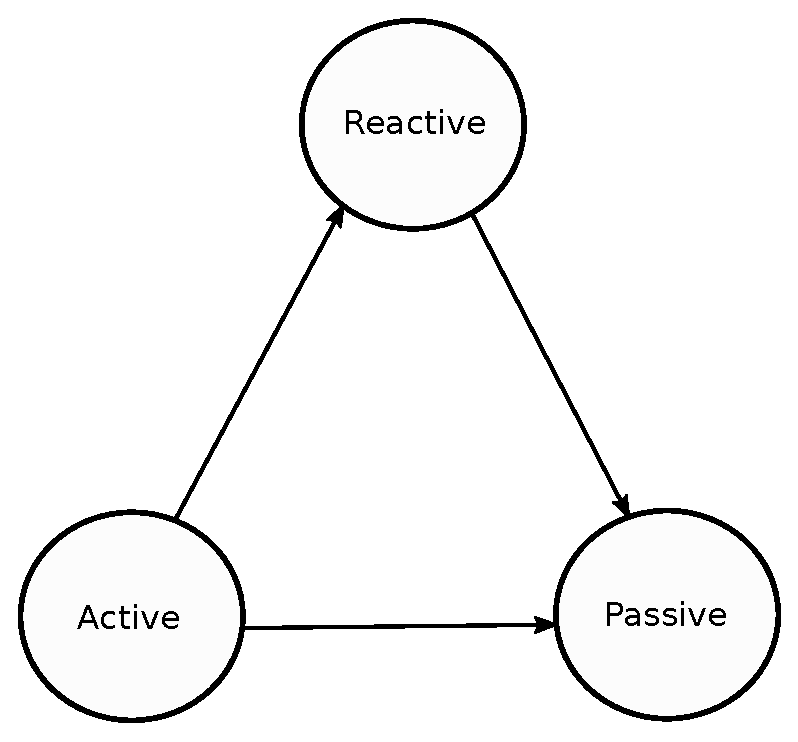
\includegraphics[width=.35\columnwidth]{sections/images/solution/entity_type_dependency.eps}
  \caption{Dependencies between entity types}
  \label{fig:sd-entity-types-deps}
\end{figure}

\subsubsection{Architectural Design}
Overview of the application layer: the classes have been divided according to 
\ref{tab:entity_type}.
\begin{figure}[H]
  \centering
  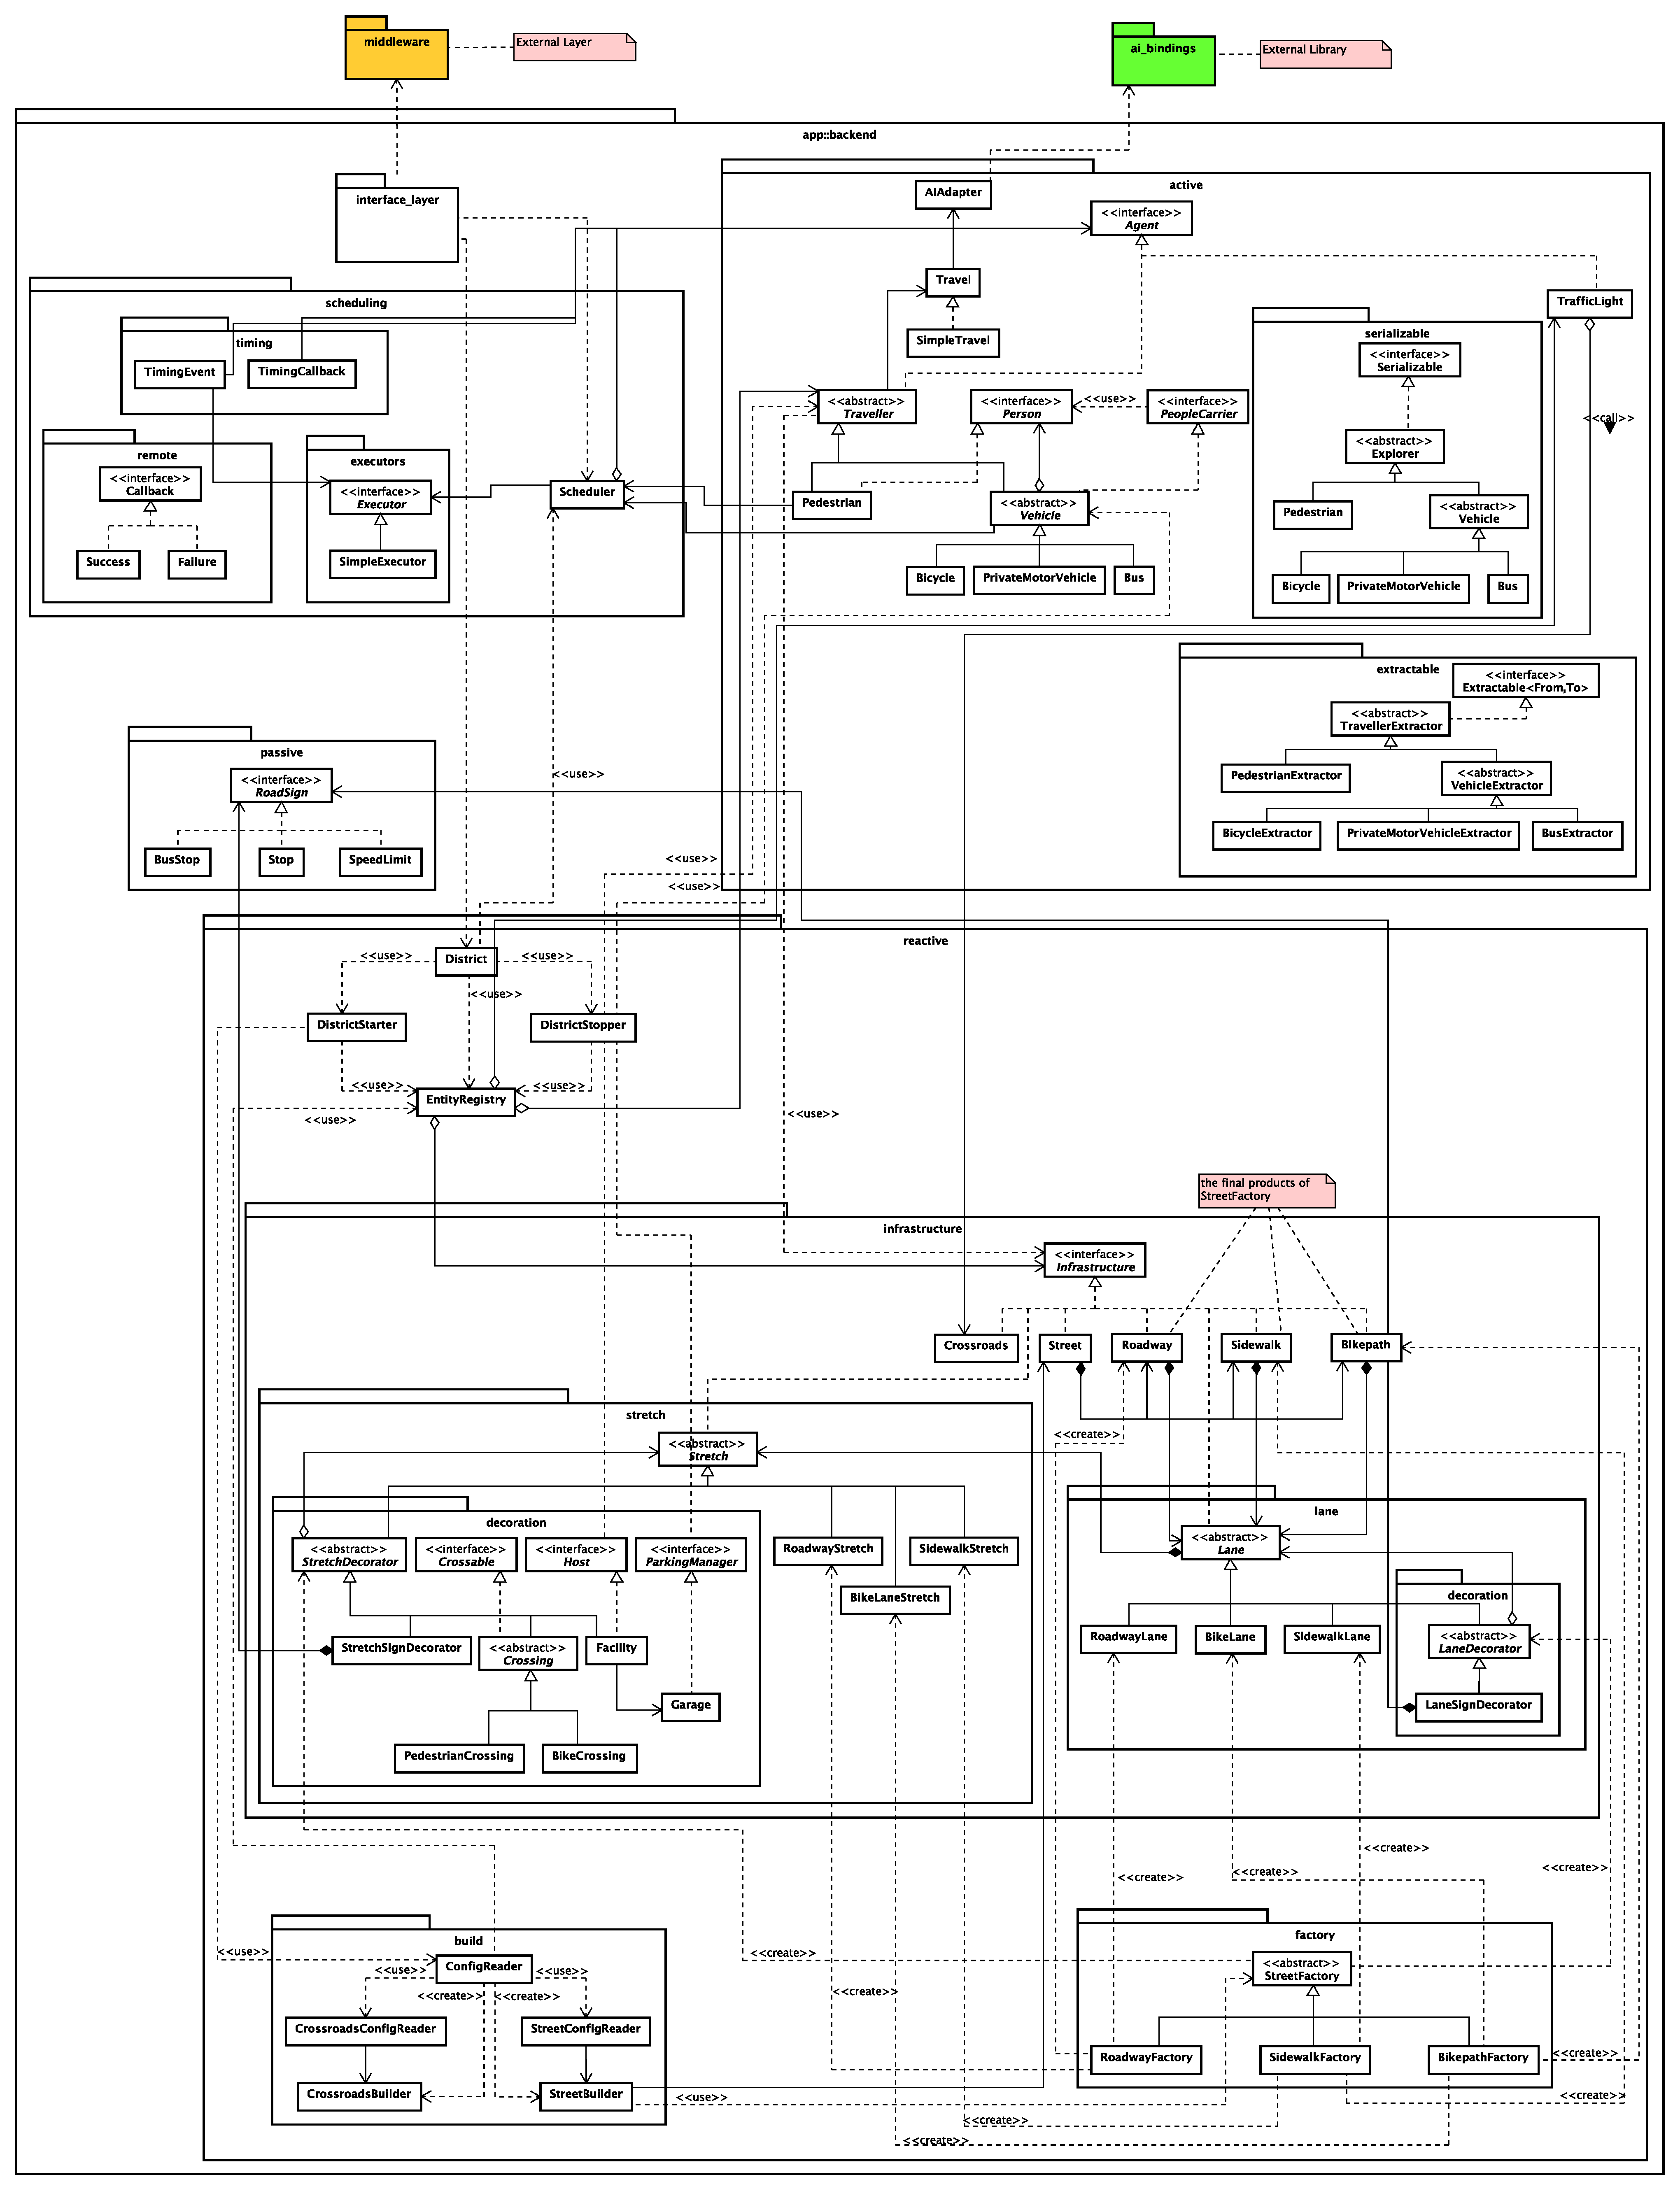
\includegraphics[width=.95\columnwidth]{images/solution/app/backend/app_backend_architecture.eps}
  \caption{Application Layer: top level design}
  \label{fig:sd-app-backend-architecture}
\end{figure}


\subsubsection{Detailed Design}
\subsubsubsection{Interface}
\subsubsubsubsection{Application}
\begin{figure}[h]
\centering
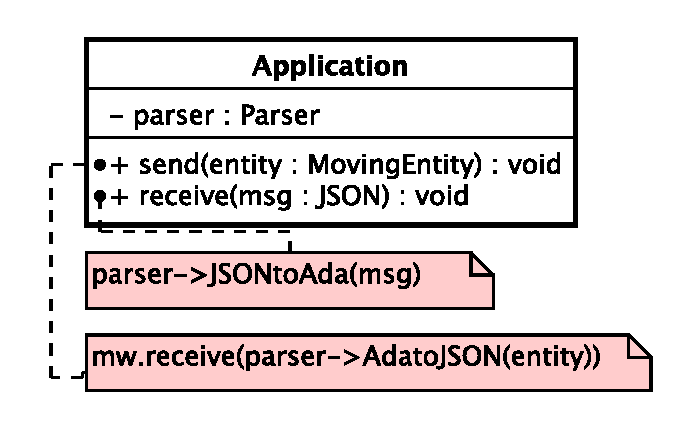
\includegraphics[scale=0.6,keepaspectratio]{images/solution/application.eps}
\caption{App::Interface::Application}
\label{fig:sd-app-application}
\end{figure}
\FloatBarrier
\begin{itemize}
  \item \textbf{Description} \\
    It represents a lightweight interface to communicate with the middleware layer.
  \item \textbf{Attribute}
  \begin{itemize}
    \item \texttt{- parser: Parser} \\
The parser object used to convert JSON data to Ada instructions and vice versa.
  \end{itemize}
  \item \textbf{Operation}
  \begin{itemize} 
    \item \texttt{+ send(entity: MovingEntity)} \\
Sends messages to the middleware layer. Before sending the message to the
middleware it converts the entity into a JSON message using the parser.
    \item \texttt{+ receive(msg: JSON)} \\
Receives a JSON messae from the middleware layer. It invokes the parser 
passing the message as parameter.
  \end{itemize}
\end{itemize}

\subsubsubsubsection{Parser}
\begin{figure}[h]
\centering
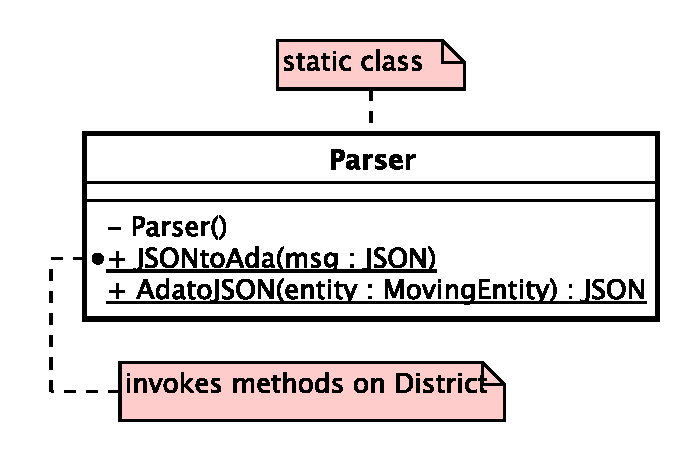
\includegraphics[scale=0.6,keepaspectratio]{images/solution/parser.eps}
\caption{App::Active::Parser}
\label{fig:sd-app-parser}
\end{figure}
\FloatBarrier
\begin{itemize}
  \item \textbf{Description} \\
    It represents a parser which converts JSON messages to Ada statements and vice versa.
  \item \textbf{Attribute}
  \begin{itemize}
    \item \texttt{- district: District} \\
The district object used as facade for the application layer.
  \end{itemize}
  \item \textbf{Operation}
  \begin{itemize} 
    \item \texttt{+ JSONtoAda(msg: JSON)} \\
Converts the JSON message to Ada statements invoking district.
    \item \texttt{+ AdatoJSON(entity: MovingEntity) : JSON} \\
Converts a moving entity into a JSON message returning the message as result.
  \end{itemize}
\end{itemize}

\subsubsubsection{Active Entity}
\subsubsubsubsection{Moving entity}
\begin{figure}[h]
\centering
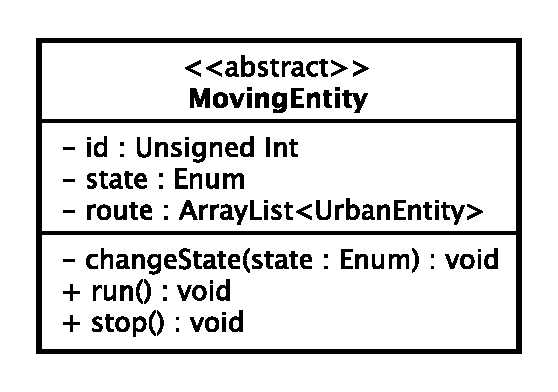
\includegraphics[scale=0.6,keepaspectratio]{images/solution/moving_entity.eps}
\caption{App::Active::MovingEntity}
\label{fig:sd-app-movingentity}
\end{figure}
\FloatBarrier
\begin{itemize}
  \item \textbf{Description} \\
    It represents an entity that moves through the city, consuming its 
route at each stretch treaded.
  \item \textbf{Attribute}
  \begin{itemize}
    \item \texttt{- id: Unsigned Int} \\
A unique identifier, useful to keep track of each entity.
    \item \texttt{- state: Enum} \\
The possible states of the entity \{ running, stopped \}.
    \item \texttt{- route: ArrayList<UrbanEntity>} \\
The route of urban entities that the entity has to tread.
    \item \texttt{- maxSpeed: Unsigned Int} \\
The maximum possible speed for the entity.
  \end{itemize}
  \item \textbf{Operation}
  \begin{itemize}
    \item \texttt{- changeState(state: Enum)} \\
Change the entity state. This method is used internally by public methods to 
change the entity behaviour.
    \item \texttt{- setSpeedLimit(speed: Unsigned Int)} \\
Updates the maximum speed of the entity.
    \item  \texttt{+ MovingEntity(route: ArrayList<UrbanEntity>)} \\
Creates a moving entity setting its route.
    \item  \texttt{+ run()} \\
Activates the entity which sets its state to \textit{running} and 
starts consuming its route.
    \item  \texttt{+ stop()} \\
Stops the entity which sets its state to \textit{stopped}.
   \item  \texttt{+ getMaxSpeed() : Unsigned Int} \\
Returns the maximum speed of the entity.
     \item  \texttt{+ getId() : Unsigned Int} \\
Returns the id of the entity. 
    \item  \texttt{+ notify(house: House) : ArrayList<Pedestrian>} \\
Decide if it want to rest in the house according to its route: in this case
returns a list of pedestrian which wants to stay in the house, otherwise returns
an empty list.
    \item  \texttt{+ update(roadsign: RoadSign) : boolean} \\
Check the road sign concrete type and then behaves according to it (i.e. if the
road sign is a speed limit it updates its maxSpeed using this.setSpeedLimit(roadsign.getLimit())). Returns true if completed correctly/action accepted, false otherwise.
  \end{itemize}
\end{itemize}

\subsubsubsubsection{Vehicle}
\begin{figure}[h]
\centering
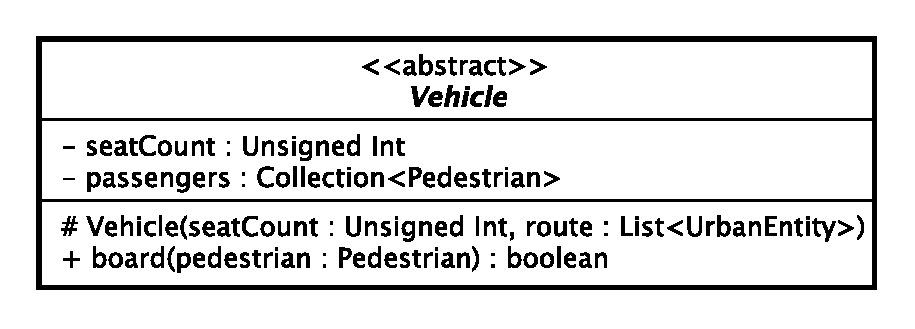
\includegraphics[scale=0.6,keepaspectratio]{images/solution/vehicle.eps}
\caption{App::Active::Vehicle}
\label{fig:sd-app-vehicle}
\end{figure}
\begin{itemize}
  \item \textbf{Description} \\
    It represents an entity that moves through the city carrying one or more
pedestrians.
  \item \textbf{Attribute}
  \begin{itemize}
    \item \texttt{- maxSeats: Unsigned Int} \\
The maximum number of seats in the vehicle.
    \item \texttt{- seat: ArrayList<Pedestrian>} \\
The list of passengers carried by the vehicle.
  \end{itemize}
  \item \textbf{Operation}
  \begin{itemize} 
    \item \texttt{+ Vehicle(maxSeats: Unsigned Int)} \\
Creates a vehicle specifying its maximum number of seats.
    \item \texttt{+ board(passenger: Pedestrian) : boolean} \\
If the vehicle is not full the pedestrian become a passenger and the method 
returns \textit{true}. Otherwise the access to the vehicle is not granted and 
the method returns false.
  \end{itemize}
\end{itemize}

\subsubsubsubsection{ConcreteVehicle}
\begin{figure}[h]
\centering
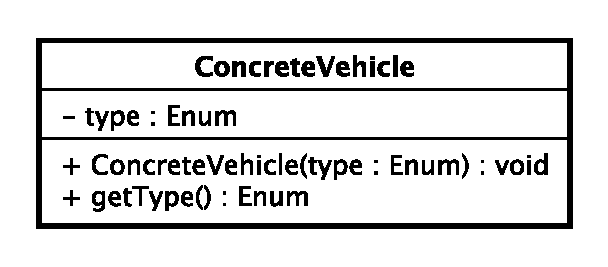
\includegraphics[scale=0.6,keepaspectratio]{images/solution/concrete_vehicle.eps}
\caption{App::Active::ConcreteVehicle}
\label{fig:sd-app-concrete-vehicle}
\end{figure}
\FloatBarrier
\begin{itemize}
  \item \textbf{Description} \\
It represents an entity that moves only on roadways.
  \item \textbf{Attribute}
  \begin{itemize}
    \item \texttt{- type: Enum} \\
Each vehicle has a type \{ car, motorcycle, sidecar \}.
  \end{itemize}
  \item \textbf{Operation}
  \begin{itemize} 
    \item \texttt{+ ConcreteVehicle(type: Enum)} \\
Creates a vehicle specifying its type.
    \item \texttt{+ getType() : Enum} \\
Returns the type of the concrete vehicle.
  \end{itemize}
\end{itemize} 

\subsubsubsubsection{Bicycle}
\begin{figure}[h]
\centering

\includegraphics[scale=0.6,keepaspectratio]{images/solution/bicycle.eps}
\caption{App::Active::Bicycle}
\label{fig:sd-app-bicycle}
\end{figure}
\FloatBarrier
\begin{itemize}
  \item \textbf{Description} \\
It represents an entity that moves only on bikepaths.
\end{itemize} 

\subsubsubsubsection{Bus}
\begin{figure}[h]
\centering
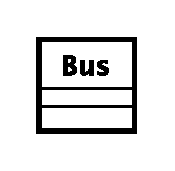
\includegraphics[scale=0.6,keepaspectratio]{images/solution/bus.eps}
\caption{App::Active::Bus}
\label{fig:sd-app-bus}
\end{figure}
\FloatBarrier
\begin{itemize}
  \item \textbf{Description} \\
It represents an entity that moves only on roadways and stops at each bus stop to
wait for passengers.
\end{itemize} 

\subsubsubsubsection{Pedestrian}
\begin{figure}[h]
\centering
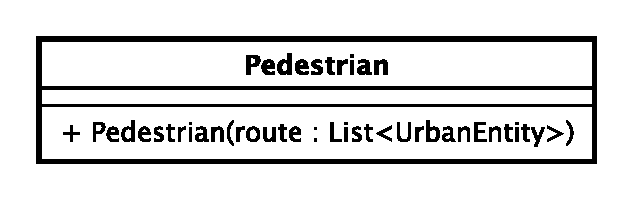
\includegraphics[scale=0.6,keepaspectratio]{images/solution/pedestrian.eps}
\caption{App::Active::Pedestrian}
\label{fig:sd-app-pedestrian}
\end{figure}
\begin{itemize}
  \item \textbf{Description} \\
It represents an entity that only moves on sidewalks.
\end{itemize} 

\subsubsubsubsection{Traffic Light}
\begin{figure}[h]
\centering
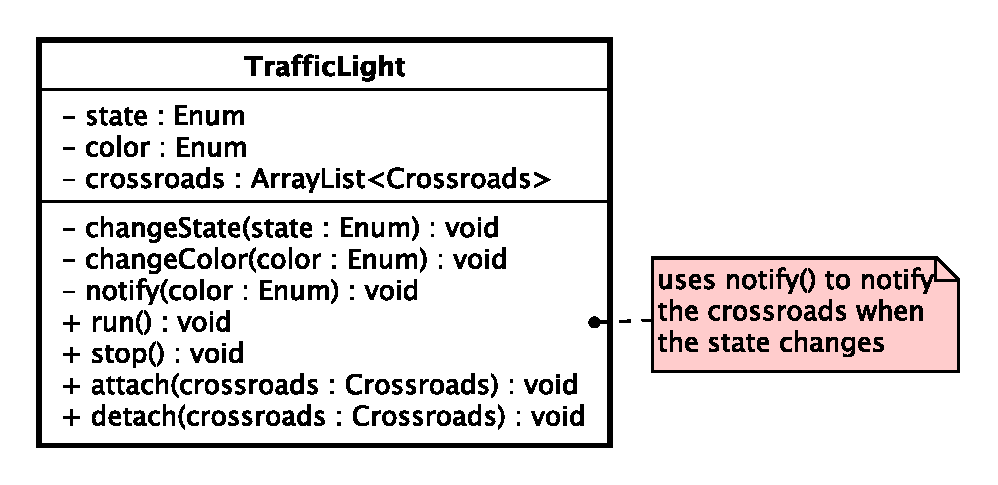
\includegraphics[scale=0.6,keepaspectratio]{images/solution/traffic_light.eps}
\caption{App::Active::TrafficLight}
\label{fig:sd-app-traffic-light}
\end{figure}
\FloatBarrier
\begin{itemize}
  \item \textbf{Description} \\
    It represents an entity that has two possible colors (green, red) and switch
between them after a specified period of time.
  \item \textbf{Attribute}
  \begin{itemize}
    \item \texttt{- state: Enum} \\
The possible states of the entity \{ running, stopped \}.
    \item \texttt{- color: Enum} \\
The possible colors of the entity \{ green, red \}.
  \end{itemize}
  \item \textbf{Operation}
  \begin{itemize} 
    \item \texttt{- changeState(state: Enum)} \\
Change the entity state. This method is used internally by public methods to 
change the entity behaviour.
    \item \texttt{- changeColor(color: Enum)} \\
Change the entity color. This method is used internally by public methods to 
switch between entity colors.
    \item \texttt{+ run(crossroads: Crossroads)} \\
Activates the entity which sets its state to \textit{running}. If its color is 
\textit{green} then it notifies the crossroads and then changes its color, 
otherwise it changes its color to \textit{green} and then notifies 
the crossroad. After changing its color it waits for n seconds.    
    \item \texttt{+ stop()} \\
Stops the entity which sets its state to \textit{stopped}.
  \end{itemize}
\end{itemize}

\subsubsubsection{ReactiveEntity}
\subsubsubsubsection{District}
\begin{figure}[h]
\centering
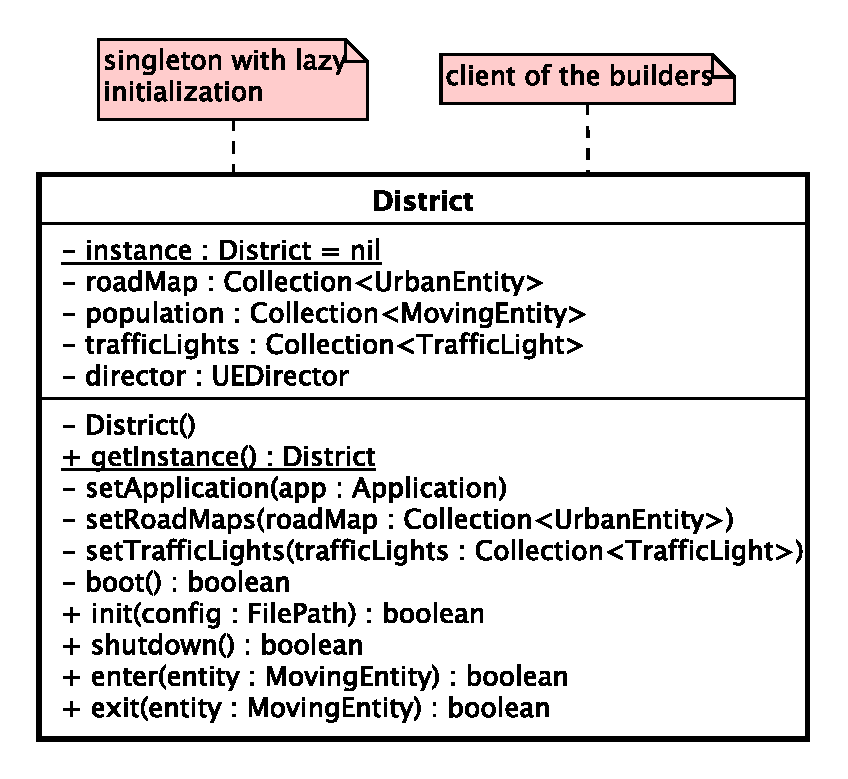
\includegraphics[scale=0.6,keepaspectratio]{images/solution/district.eps}
\caption{App::Reactive::District}
\label{fig:sd-app-district}
\end{figure}
\FloatBarrier
\begin{itemize}
  \item \textbf{Description} \\
It represents the master entity of the application layer. 
It has the responsibility to boot and shutdown the application layer.
  \item \textbf{Attribute}
  \begin{itemize}
    \item \texttt{- app: Application} \\
A reference to the interface of the application layer.
    \item \texttt{- roadMap: ArrayList<UrbanEntity>} \\
The urban entities of the district\footnote{Note that the name 
\textit{district} is only a convetion, indeed it is possible to have a 
real district splitted into different logical nodes of the system}
(i.e. crossroads and streets). 
    \item \texttt{- population: ArrayList<MovingEntity>} \\
The moving entities that reside on the district.
    \item \texttt{- trafficLight: ArrayList<TrafficLight>} \\
The traffic lights of the district.
    \item \texttt{- director: UEDirector} \\ 
The director of the city building process.
  \end{itemize}
  \item \textbf{Operation}
  \begin{itemize} 
    \item \texttt{- boot() : boolean} \\
Boots the application layer running all the active entities of the 
district (moving entities and traffic lights).
Returns true if the process completes neatly, false otherwise. 
This method is internally used by init.
    \item \texttt{+ init(config: FilePath) : boolean} \\
Creates and boots all the entities of the district according to the 
configuration file. Attaches each crossroads to the relative traffic light
if specified so in the configuration file. 
Returns true if the process completes neatly, false otherwise.
    \item \texttt{+ shutdown() : boolean} \\
Terminates the district. Returns true if the process completes neatly,
false otherwise.
    \item \texttt{+ enter(entity: MovingEntity) : boolean} \\
Notifies the district to add a new moving entity to the population.
Returns true if the process completes neatly, false otherwise.
    \item \texttt{+ exit(entity: MovingEntity) : boolean} \\
Notifies the district to pass a moving entity from the roadMap to the 
application layer interface which communicates to the middleware layer.
Returns true if the process completes neatly, false otherwise.
  \end{itemize}
\end{itemize} 

\subsubsubsubsection{UEDirector}
\begin{figure}[h]
\centering
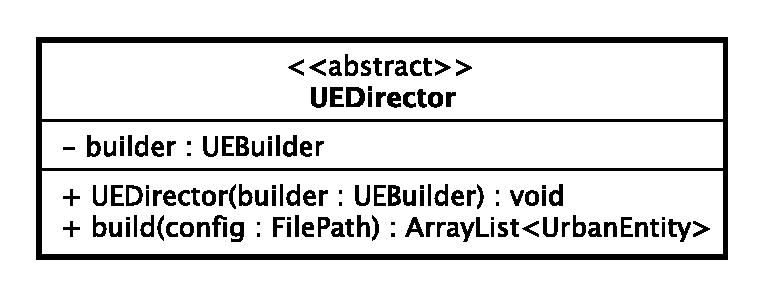
\includegraphics[scale=0.6,keepaspectratio]{images/solution/uedirector.eps}
\caption{App::Reactive::UEDirector}
\label{fig:sd-app-uedirector}
\end{figure}
\FloatBarrier
\begin{itemize}
  \item \textbf{Description} \\
    It represents the urban entity director which instructs the builder.
  \item \textbf{Attribute}
  \begin{itemize}
    \item \texttt{- builder: UEBuilder} \\
The builder object which builds parts of the district.
  \end{itemize}
  \item \textbf{Operation}
  \begin{itemize} 
    \item \texttt{+ UEDirector(builder: UEBuilder)} \\
Creates a director with its own builder object.
    \item \texttt{+ build(config: FilePath) : ArrayList<UrbanEntity>} \\
Builds a list of urban entities according to the configuration file. It uses the
builder multiple times to create incrementally a specific configuration of the
requested urban entity specified in the configuration file. 
  \end{itemize}
\end{itemize}

\subsubsubsubsection{Crossroads Director}
\begin{figure}[h]
\centering
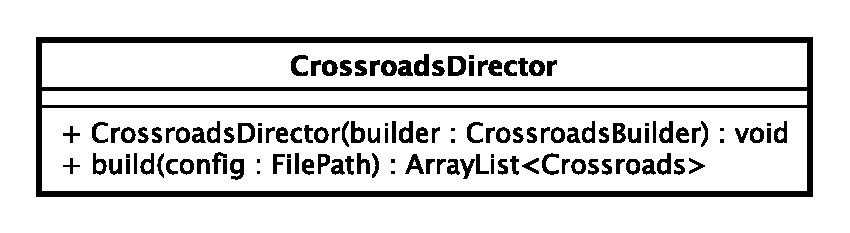
\includegraphics[scale=0.6,keepaspectratio]{images/solution/crossroads_director.eps}
\caption{App::Reactive::Crossroads Director}
\label{fig:sd-app-crossroads_director}
\end{figure}
\FloatBarrier
\begin{itemize}
  \item \textbf{Description} \\
    It represents the concrete director of the crossroads builder.
  \item \textbf{Operation}
  \begin{itemize} 
    \item \texttt{+ CrossroadsDirector(builder: CrossroadsBuilder)} \\
Creates a concrete crossroads director with its own crossroads builder.
    \item \texttt{+ build(config: FilePath) : ArrayList<Crossroads>} \\
Builds a list of crossroads according to the configuration file. 
It uses the builder multiple times 
to create incrementally a configuration of the requested crossroads as specified
in the configuration file. 
  \end{itemize}
\end{itemize}

\subsubsubsubsection{Street Director}
\begin{figure}[h]
\centering
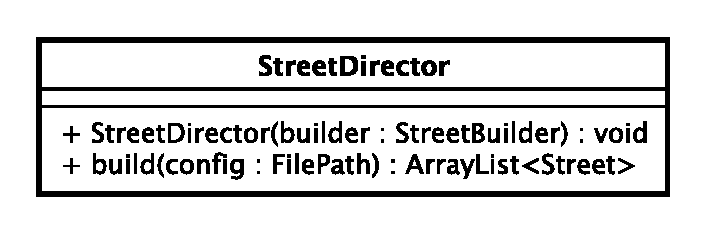
\includegraphics[scale=0.6,keepaspectratio]{images/solution/street_director.eps}
\caption{App::Reactive::Street Director}
\label{fig:sd-app-street_director}
\end{figure}
\FloatBarrier
\begin{itemize}
  \item \textbf{Description} \\
    It represents the concrete director of the street builder.
  \item \textbf{Operation}
  \begin{itemize} 
    \item \texttt{+ StreetDirector(builder: StreetBuilder)} \\
Creates a concrete street director with its own street builder.
    \item \texttt{+ build(config: FilePath) : ArrayList<Street>} \\
Builds a list of streets according to the configuration file. 
It uses the builder multiple times to create incrementally a 
specific configuration of the requested street specified 
in the configuration file. 
  \end{itemize}
\end{itemize}

\subsubsubsubsection{UEBuilder}
\begin{figure}[h]
\centering
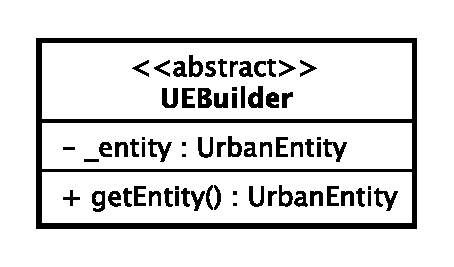
\includegraphics[scale=0.6,keepaspectratio]{images/solution/uebuilder.eps}
\caption{App::Reactive::UEBuilder}
\label{fig:sd-app-uebuilder}
\end{figure}
\FloatBarrier
\begin{itemize}
  \item \textbf{Description} \\
    It represents an entity that moves through the city carrying one or more
pedestrians.
  \item \textbf{Attribute}
  \begin{itemize}
    \item \texttt{- \_entity: UrbanEntity} \\
The entity which the builder incrementally constructs.
  \end{itemize}
  \item \textbf{Operation}
  \begin{itemize} 
    \item \texttt{+ getEntity() : UrbanEntity} \\
Returns the final product of the building.
  \end{itemize}
\end{itemize}

\subsubsubsubsection{CrossroadsBuilder}
\begin{figure}[h]
\centering
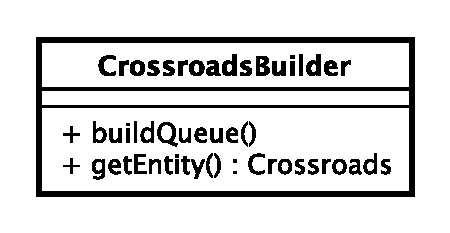
\includegraphics[scale=0.6,keepaspectratio]{images/solution/crossroads_builder.eps}
\caption{App::Reactive::CrossroadsBuilder}
\label{fig:sd-app-crossroads_builder}
\end{figure}
\FloatBarrier
\begin{itemize}
  \item \textbf{Description} \\
    It represents the builder of crossroads entities. 
  \item \textbf{Operation}
  \begin{itemize} 
    \item \texttt{+ buildTrafficLight()} \\
Adds a new traffic light to the crossroads.
    \item \texttt{+ buildQueue()} \\
Adds a new queue of moving entities to the crossroads.
    \item \texttt{+ getEntity() : Crossroads} \\
Returns the crossroads.
  \end{itemize}
\end{itemize}

\subsubsubsubsection{StreetBuilder}
\begin{figure}[h]
\centering
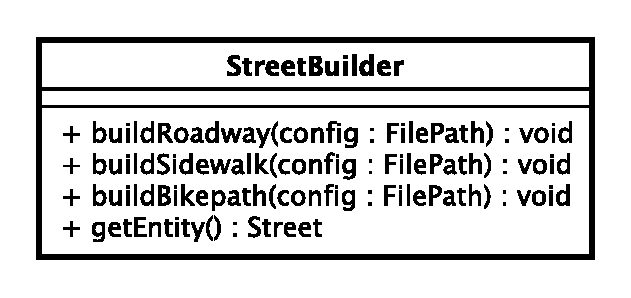
\includegraphics[scale=0.6,keepaspectratio]{images/solution/street_builder.eps}
\caption{App::Reactive::StreetBuilder}
\label{fig:sd-app-street_builder}
\end{figure}
\FloatBarrier
\begin{itemize}
  \item \textbf{Description} \\
    It represents the builder of street entities. 
  \item \textbf{Operation}
  \begin{itemize} 
    \item \texttt{+ buildRoadway(config: FilePath)} \\
Builds a roadway using roadwayfactory according to a specific configuration.
    \item \texttt{+ buildSidewalk(config: FilePath)} \\
Builds a sidewalk using sidewalkfactory according to a specific configuration.
    \item \texttt{+ buildBikepath(config: FilePath)} \\
Builds a bikepath using bikepathfactory according to a specific configuration.
    \item \texttt{+ getEntity() : Street} \\
Returns the street.
  \end{itemize}
\end{itemize}

\subsubsubsubsection{Urban Entity}
\begin{figure}[h]
\centering
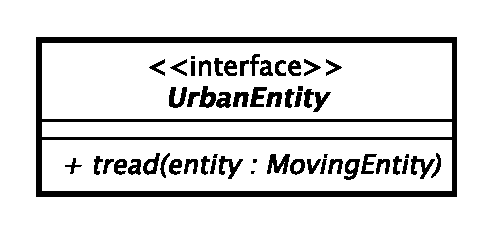
\includegraphics[scale=0.6,keepaspectratio]{images/solution/urban_entity.eps}
\caption{App::Reactive::Urban Entity}
\label{fig:sd-app-urban-entity}
\end{figure}
\FloatBarrier
\begin{itemize}
  \item \textbf{Description} \\
    It represents one of the entities the district infrastructure is composed
    of.
  \item \textbf{Operation}
  \begin{itemize} 
    \item \texttt{\textit{+ tread(entity: MovingEntity)}} \\
    Abstract method through which the urban infrastructure can be treaded by a
    moving entity.
  \end{itemize}
\end{itemize}

\subsubsubsubsection{Crossroads}
\begin{figure}[h]
\centering
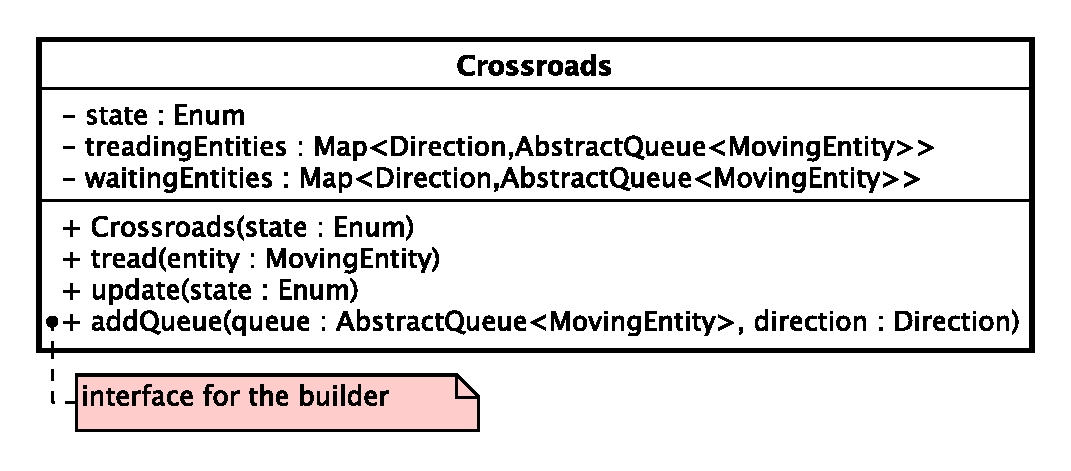
\includegraphics[scale=0.6,keepaspectratio]{images/solution/crossroads.eps}
\caption{App::Reactive::Crossroads}
\label{fig:sd-app-crossroads}
\end{figure}
\FloatBarrier
\begin{itemize}
  \item \textbf{Description} \\
    It represents a concrete crossroads entity. It is a protected object.
  \item \textbf{Attribute}
  \begin{itemize}
    \item \texttt{- state: Enum} \\
The traffic light state indicates which directions to free.
    \item \texttt{- treading: Map<Direction, AbstractQueue<MovingEntity>>} \\
The queue of moving entities which are treading the crossroads.
    \item \texttt{- waiting: Map<Direction, AbstratQueue<MovingEntity>>} \\
The queue of moving entities which are waiting to tread the crossroads. 
  \item \textbf{Operation}
  \begin{itemize} 
    \item \texttt{+ tread(entity: MovingEntity)} \\
Implements the treading of the crossroads.
    \item \texttt{+ update(state: Enum)} \\
Updates the state value of the crossroads.
    \item \texttt{+ addQueue(queue: AbstratQueue<MovingEntity>, direction: Direction)} \\
Add a new queue to waiting and treading maps with the specified direction.
  \end{itemize}
\end{itemize}

\subsubsubsubsection{Direction}
\begin{figure}[h]
\centering
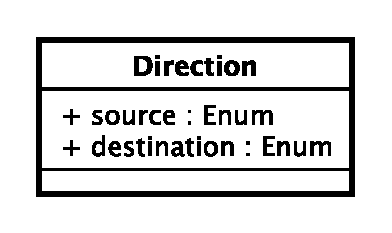
\includegraphics[scale=0.6,keepaspectratio]{images/solution/direction.eps}
\caption{App::Reactive::Direction}
\label{fig:sd-app-direction}
\end{figure}
\FloatBarrier
\begin{itemize}
  \item \textbf{Description} \\
    It represents the direction. 
  \item \textbf{Attribute}
  \begin{itemize}
    \item \texttt{- source: Enum} \\
The source from which an entity arrives. It has four possible
values \{ north, south, east, west \}
    \item \texttt{- destination: Enum} \\
The destination where the entity is directed. It has the same possible
values of source.
  \end{itemize}
\end{itemize}

\subsubsubsubsection{Street Factory}
\begin{figure}[h]
\centering
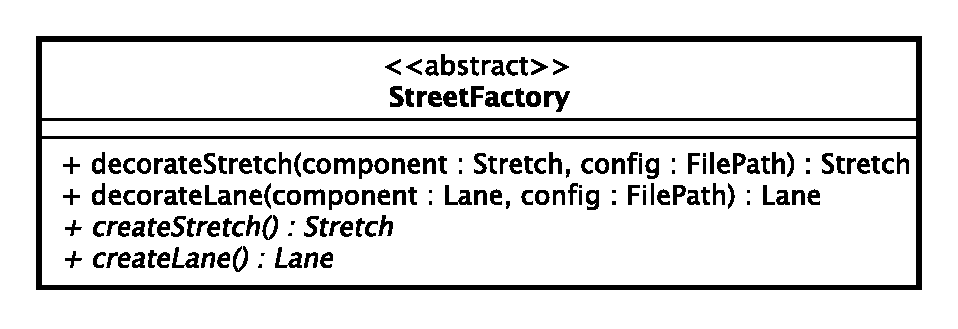
\includegraphics[scale=0.6,keepaspectratio]{images/solution/street_factory.eps}
\caption{App::Reactive::StreetFactory}
\label{fig:sd-app-street-factory}
\end{figure}
\FloatBarrier
\begin{itemize}
  \item \textbf{Description} \\
    It represents the base class of the abstract factory pattern. The 
not abstract methods of this class are used by StreetBuilder during the
building phase.
  \item \textbf{Operation} \\
  \begin{itemize} 
    \item \texttt{+ decorateStretch(component: Stretch, config: FilePath)} \\
Decorates an existing stretch component according to the configuration file parameters.
    \item \texttt{+ decorateLane(component: Lane, config: FilePath)} \\
Decorates an existing lane component according to the configuration file parameters.
    \item \texttt{\textit{+ createStretch() : Stretch}} \\
Abstract method which will create a new stretch component.
    \item \texttt{\textit{+ createLane() : Lane}} \\
Abstract method which will create a new lane component.
  \end{itemize}
\end{itemize}

\subsubsubsubsection{Roadway Factory}
\begin{figure}[h]
\centering
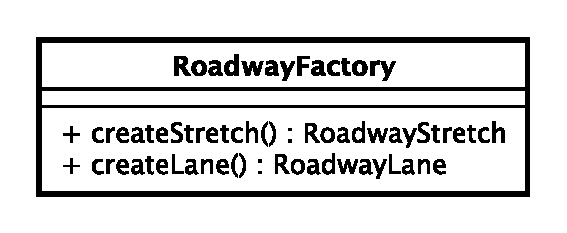
\includegraphics[scale=0.6,keepaspectratio]{images/solution/roadway_factory.eps}
\caption{App::Reactive::RoadwayFactory}
\label{fig:sd-app-roadway-factory}
\end{figure}
\FloatBarrier
\begin{itemize}
  \item \textbf{Description} \\
It represents a factory which creates roadway components.
  \item \textbf{Operation} \\
  \begin{itemize} 
    \item \texttt{+ createStretch() : RoadwayStretch} \\
Creates a new roadway stretch component.
    \item \texttt{+ createLane() : RoadwayLane} \\
Creates a new roadway lane component.
  \end{itemize}
\end{itemize}

\subsubsubsubsection{Sidewalk Factory}
\begin{figure}[h]
\centering
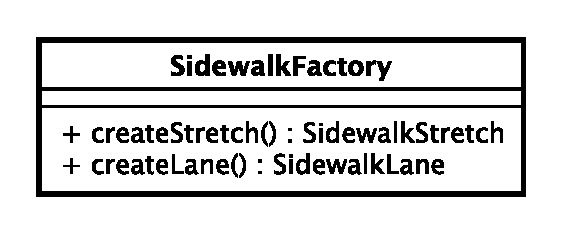
\includegraphics[scale=0.6,keepaspectratio]{images/solution/sidewalk_factory.eps}
\caption{App::Reactive::SidewalkFactory}
\label{fig:sd-app-sidewalk-factory}
\end{figure}
\FloatBarrier
\begin{itemize}
  \item \textbf{Description} \\
It represents a factory which creates sidewalk components.
  \item \textbf{Operation} \\
  \begin{itemize} 
    \item \texttt{+ createStretch() : SidewalkStretch} \\
Creates a new sidewalk stretch component.
    \item \texttt{+ createLane() : SidewalkLane} \\
Creates a new sidewalk lane component.
  \end{itemize}
\end{itemize}

\subsubsubsubsection{Bikepath Factory}
\begin{figure}[h]
\centering
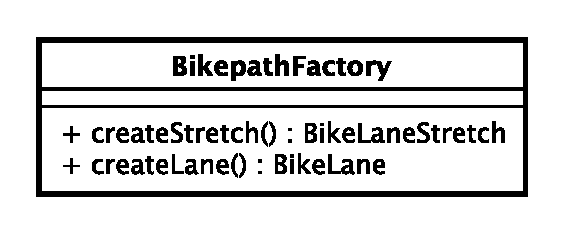
\includegraphics[scale=0.6,keepaspectratio]{images/solution/bikepath_factory.eps}
\caption{App::Reactive::BikepathFactory}
\label{fig:sd-app-bikepath-factory}
\end{figure}
\FloatBarrier
\begin{itemize}
  \item \textbf{Description} \\
It represents a factory which creates bikepath components.
  \item \textbf{Operation} \\
  \begin{itemize} 
    \item \texttt{+ createStretch() : BikeLaneStretch} \\
Creates a new bike lane stretch component.
    \item \texttt{+ createLane() : BikeLane} \\
Creates a new bike lane component.
  \end{itemize}
\end{itemize}

\subsubsubsubsection{Street}
\begin{figure}[h]
\centering
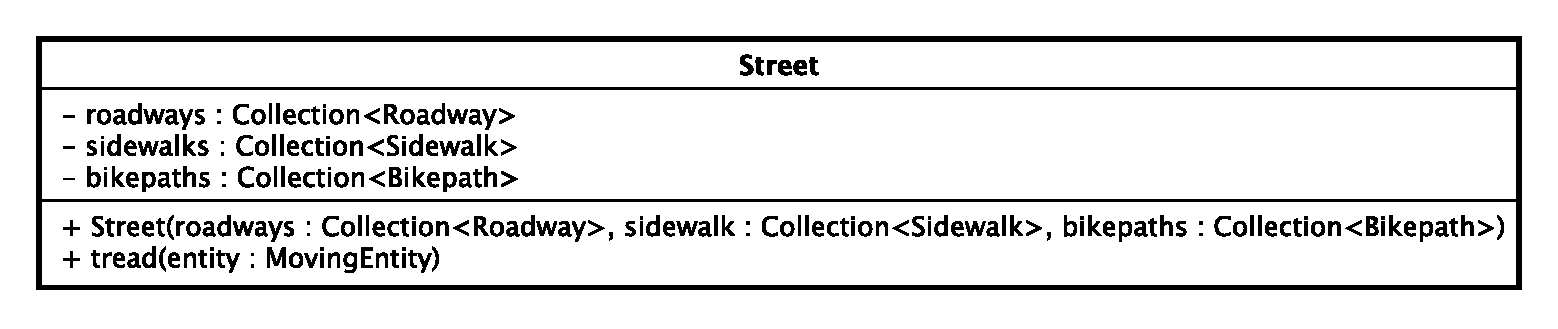
\includegraphics[scale=0.6,keepaspectratio]{images/solution/street.eps}
\caption{App::Reactive::Street}
\label{fig:sd-app-street}
\end{figure}
\FloatBarrier
\begin{itemize}
  \item \textbf{Description} \\
    It represents a concrete street.
  \item \textbf{Attribute}
  \begin{itemize}
    \item \texttt{- roadway: ArrayList<Roadway>} \\
A street has a roadway.
    \item \texttt{- sidewalk: ArrayList<Sidewalk>} \\
A street can have one or more sidewalks (typically one for each side
of the street).
    \item \texttt{- bikepath: ArrayList<Bikepath>} \\
A street can have one or more bikepaths, (typically one for each side
of the street).
  \end{itemize}
  \item \textbf{Operation}
  \begin{itemize} 
    \item \texttt{+ tread(entity: MovingEntity)} \\
Moves the entity in the proper part of the street based on the
concrete type of the entity (i.e. pedestrians will move on sidewalks).
  \end{itemize}
\end{itemize}

\subsubsubsubsection{Roadway}
\begin{figure}[h]
\centering
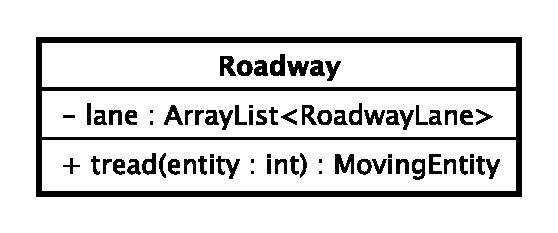
\includegraphics[scale=0.6,keepaspectratio]{images/solution/roadway.eps}
\caption{App::Reactive::Roadway}
\label{fig:sd-app-roadway}
\end{figure}
\FloatBarrier
\begin{itemize}
  \item \textbf{Description} \\
    It represents a concrete roadway which is composed of one or more lanes.
  \item \textbf{Attribute}
  \begin{itemize}
    \item \texttt{- lane: ArrayList<RoadwayLane>} \\
A roadway is composed of lanes.
  \end{itemize}
  \item \textbf{Operation}
  \begin{itemize} 
    \item \texttt{+ tread(entity: MovingEntity)} \\
Moves the entity on the correct lane based on the current entity route. 
  \end{itemize}
\end{itemize}

\subsubsubsubsection{Bikepath}
\begin{figure}[h]
\centering
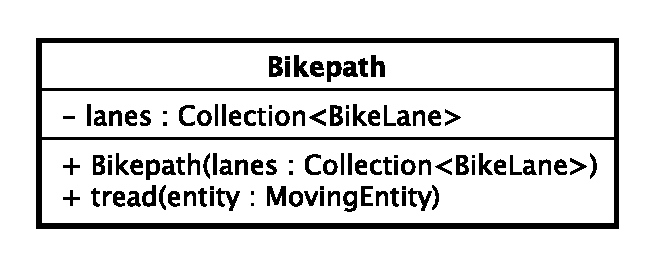
\includegraphics[scale=0.6,keepaspectratio]{images/solution/bikepath.eps}
\caption{App::Reactive::Bikepath}
\label{fig:sd-app-bikepath}
\end{figure}
\FloatBarrier
\begin{itemize}
  \item \textbf{Description} \\
    It represents a concrete bikepath which is composed by at least one lane.
  \item \textbf{Attribute}
  \begin{itemize}
    \item \texttt{- lane: ArrayList<BikeLane>} \\
A bikepath is composed by lanes.
  \end{itemize}
  \item \textbf{Operation}
  \begin{itemize} 
    \item \texttt{+ tread(entity: MovingEntity)} \\
Moves the entity on the correct lane based on the current entity route. 
  \end{itemize}
\end{itemize}

\subsubsubsubsection{Sidewalk}
\begin{figure}[h]
\centering
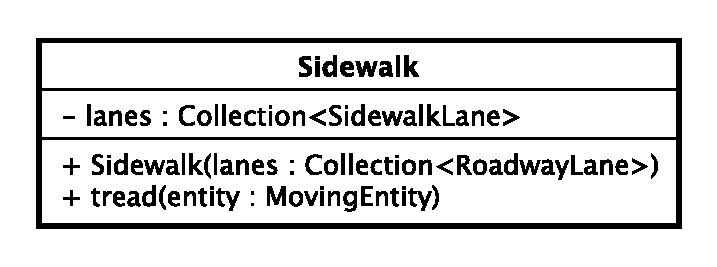
\includegraphics[scale=0.6,keepaspectratio]{images/solution/sidewalk.eps}
\caption{App::Reactive::Sidewalk}
\label{fig:sd-app-sidewalk}
\end{figure}
\FloatBarrier
\begin{itemize}
  \item \textbf{Description} \\
    It represents a concrete sidewalk which is composed by at least one lane.
  \item \textbf{Attribute}
  \begin{itemize}
    \item \texttt{- lane: ArrayList<SidewalkLane>} \\
A sidewalk is composed by lanes.
  \end{itemize}
  \item \textbf{Operation}
  \begin{itemize} 
    \item \texttt{+ tread(entity: MovingEntity)} \\
Moves the entity on the correct lane based on the current entity route. 
  \end{itemize}
\end{itemize}

\subsubsubsubsection{Lane}
\begin{figure}[h]
\centering
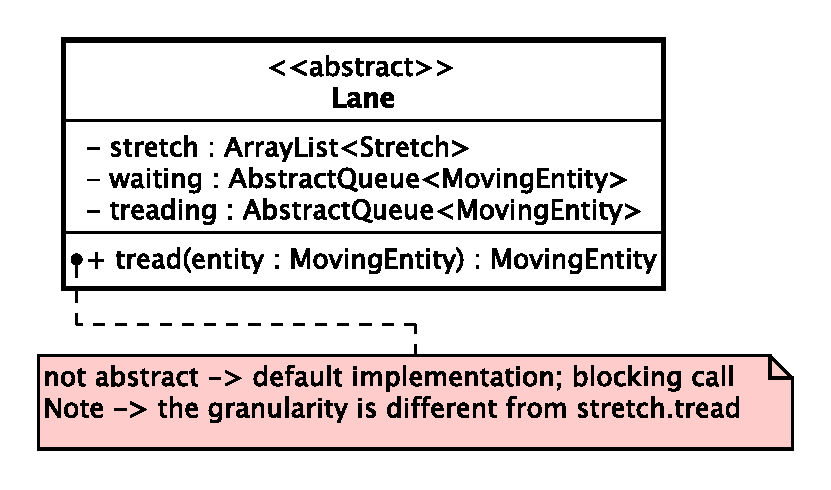
\includegraphics[scale=0.6,keepaspectratio]{images/solution/lane.eps}
\caption{App::Reactive::Lane}
\label{fig:sd-app-lane}
\end{figure}
\FloatBarrier
\begin{itemize}
  \item \textbf{Description} \\
    It represents a lane entity. It is a protected object composed of one or
    more stretches.
  \item \textbf{Attribute}
  \begin{itemize}
    \item \texttt{- size: Unsigned Int} \\
The size of the stretch/treading queue.
    \item \texttt{- stretch: ArrayList<Stretch>} \\
The list of stretches which compose the lane.
    \item \texttt{- treading: AbstractQueue<MovingEntity>} \\
The queue of moving entities which are treading the lane.
    \item \texttt{- waiting: AbstractQueue<MovingEntity>} \\
The queue of moving entities which are waiting to tread the lane. 
  \end{itemize}
  \item \textbf{Operation}
  \begin{itemize} 
    \item \texttt{+ Lane(size: Unsigned Int, stretch: ArrayList<Stretch>)} \\
Creates a \texttt{Lane} object with a specific size and list of stretches.
    \item \texttt{+ tread(entity: MovingEntity)} \\
Implements the lane treading. Moves the entity on the stretches which are 
in the moving entity route.
  \end{itemize}
\end{itemize}

\subsubsubsubsection{Stretch}
\begin{figure}[h]
\centering
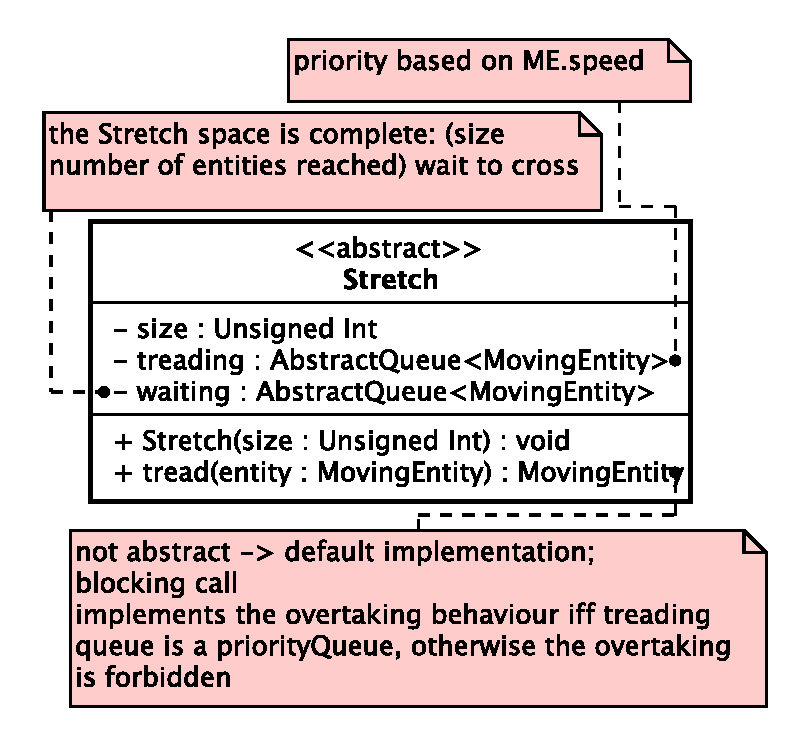
\includegraphics[scale=0.6,keepaspectratio]{images/solution/stretch.eps}
\caption{App::Reactive::Stretch}
\label{fig:sd-app-stretch}
\end{figure}
\FloatBarrier
\begin{itemize}
  \item \textbf{Description} \\
    It represents a stretch entity. It is a protected object.
  \item \textbf{Attribute}
  \begin{itemize}
    \item \texttt{- size: Unsigned Int} \\
The size of the stretch/treading queue.
    \item \texttt{- treading: AbstractQueue<MovingEntity>} \\
The queue of moving entities which are treading the stretch. If the concrete type
is PriorityQueue then the stretch allows the overtaking between the moving entities.
This is implemented through a priority queue ordered by decresing speed.
    \item \texttt{- waiting: AbstractQueue<MovingEntity>} \\
The queue of moving entities which are waiting to tread the stretch. 
  \end{itemize}
  \item \textbf{Operation}
  \begin{itemize}
    \item \texttt{+ Stretch(size: Unsigned Int)} \\
Creates a stretch object with a specific size.
    \item \texttt{+ tread(entity: MovingEntity)} \\
Implements the treading of the stretch. The current speed of the moving entity
is calculated first, then the entity is placed in a treading queue which has a  
timeout, after the deadline elapsed the queue is flushed and the entity can proceed
along their route.
  \end{itemize}
\end{itemize}

\subsubsubsubsection{Roadway Stretch}
\begin{figure}[h]
\centering
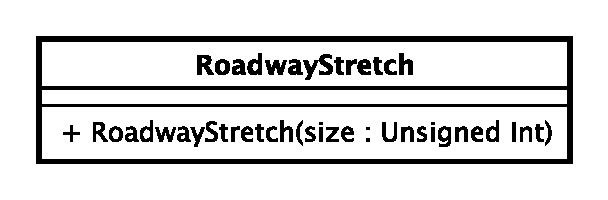
\includegraphics[scale=0.6,keepaspectratio]{images/solution/roadway_stretch.eps}
\caption{App::Reactive::RoadwayStretch}
\label{fig:sd-app-roadway_stretch}
\end{figure}
\FloatBarrier
\begin{itemize}
  \item \textbf{Description} \\
    It represents a roadway stretch entity. It is a protected object. Only specific types of vehicles can tread this kind of stretch.
\end{itemize}

\subsubsubsubsection{Bike Lane Stretch}
\begin{figure}[h]
\centering

\includegraphics[scale=0.6,keepaspectratio]{images/solution/bikelane_stretch.eps}
\caption{App::Reactive::BikeLaneStretch}
\label{fig:sd-app-bikelane_stretch}
\end{figure}
\FloatBarrier
\begin{itemize}
  \item \textbf{Description} \\
    It represents a bike lane stretch entity. It is a protected object. Only bycicles 
can tread this kind of stretch.
\end{itemize}

\subsubsubsubsection{Sidewalk Stretch}
\begin{figure}[h]
\centering
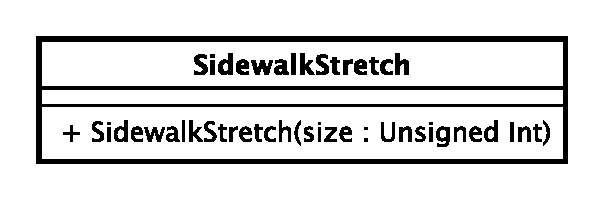
\includegraphics[scale=0.6,keepaspectratio]{images/solution/sidewalk_stretch.eps}
\caption{App::Reactive::SidewalkStretch}
\label{fig:sd-app-sidewalk_stretch}
\end{figure}
\FloatBarrier
\begin{itemize}
  \item \textbf{Description} \\
    It represents a sidewalk stretch entity. It is a protected object. Only pedestrians
can tread this kind of stretch.
\end{itemize}

\subsubsubsection{PassiveEntity}

%\subsubsection{Road}
\begin{figure}[h]
\centering
\nogloxy{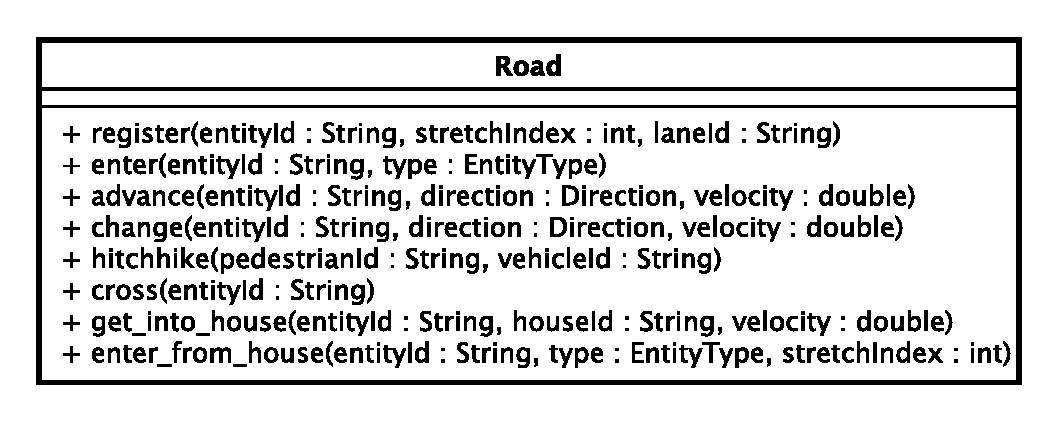
\includegraphics[scale=0.6,keepaspectratio]{diagrams/workspace/application/road.eps}}
\caption{Application::Road}
\end{figure}
\FloatBarrier
A Road is made of stretches and it offers the following operations:
\begin{itemize}
	\item \texttt{register(entityId : String, stretchIndex : int, laneId : String)}
	\\Puts an entity into the stretch having the given index
	\begin{itemize}
		\item \textit{Use}: boostrap phase
	\end{itemize}
	\item \texttt{enter(entityId : String, type : EntityType)}
	\\Puts an entity into the Road in the rightmost lane available for the entity type
	\begin{itemize}
		\item E.g. a car does not land in a sidewalk
	\end{itemize}
	\item \texttt{advance(entityId : String, direction : Direction, velocity : double)}
	\\Moves an entity forward along the Road	
	\begin{itemize}
		\item If a Road end has reached, the entity is notified providing it the adjacent Roads list
		\item The entity velocity is calculated by each stretch taking a specific range of possible values according to the entity type
	\end{itemize}
	\item \texttt{change(entityId : String, direction : Direction, velocity : double)}
	\\Moves an entity to next stretch in the given direction (left or right)	
	\begin{itemize}
		\item If a Road end is reached, it does not allow the lane change and it sends a message for notifying the entity
		\item If no more lanes for the entity type exist in the given direction, it sends a message for notifying the entity
	\end{itemize}
	\item \texttt{hitchhike(pedestrianId : String, vehicleId : String)}
	\\Brings a pedestrian into an vehicle
	\item \texttt{cross(entityId : String)}
	\\Moves a pedestrian or a cyclist to the other side of the Road
	\begin{itemize}
		\item If there is an entity in the stretch near a sidewalk, it books a Road crossing
		\item No vehicles can enter stretches covered by booked zebra crossing
		\item If a stretch near a sidewalk is free (whether it is booked or not), pedestrian can start crossing the Road
	\end{itemize}
	\item \texttt{get\_into\_house(entityId : String, houseId : String, velocity : double)}
	\\Brings an entity into a house accessible from the Road where the entity is
	\begin{itemize}
		\item It brings the entity into the house, if the entity is in a stretch where the given house is accessible. Otherwise, It moves the entity forward at the specified velocity
	\end{itemize}
	\item \texttt{enter\_from\_house(entityId : String, type : EntityType, stretchIndex : int)}
	\\Brings an entity out from a house and it puts the entity into the Road stretch having the given index
	\begin{itemize}
		\item An entity coming out from a house has lower priority than one is already on the Road. So that, before exiting the house, the first one has to wait the other one is passed
	\end{itemize}
\end{itemize}
\paragraph{Remarks}
\ \\A lane change can happen in two cases:
\begin{itemize}
	\item Overtaking. It is requested in a particular stretch
	\item Road change. It is requested in the first stretch of the Road taken
\end{itemize}
We assume a Road is at least $n$ stretches long if it consists of $n$ lanes for motor vehicles.
%\subsubsection{Semaphore}
\begin{figure}[h]
\centering
\nogloxy{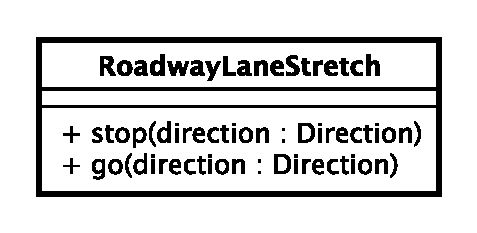
\includegraphics[scale=0.6,keepaspectratio]{diagrams/workspace/application/roadwayLaneStretch.eps}}
\caption{Application::RoadwayLaneStretch}
\end{figure}
\FloatBarrier
A semaphore is placed at the end of a roadway lane stretch offers the following operations:
\begin{itemize}
	\item \texttt{stop(direction : Direction)}
	\\Blocks outgoing flow of vehicles going towards a given direction
	\item \texttt{go(direction : Direction)}
	\\Allows outgoing flow of vehicles going towards a given direction
\end{itemize}
\paragraph{Remaks}
\ \\\texttt{stop} and \texttt{go} operations are called by a set of semaphores, that communicate internally to advance through their RGY steps.

The \texttt{direction} parameter assumes the values:
\begin{itemize}
	\item N or S  for “vertical” street
	\item W or E for “horizontal” street
\end{itemize}
%\subsubsection{Moving entity}
%TODO add Moving entity section
%\subsubsection{House}
A house (or facility) is populated by individuals (people) and it offers the following functional channels:
\begin{itemize}
	\item \texttt{register(entity, segmentIndex)}
	\\Puts an entity into a house
	\begin{itemize}
		\item \textit{use}: bootstrap phase
	\end{itemize}
\end{itemize}
Notes:
Freezing sleep could be tricky: how to save the partial timeout we reached? It could be useful to save a timestamp of sleep beginning too.
%\subsubsection{Crossroads}
\begin{figure}[h]
\centering
\nogloxy{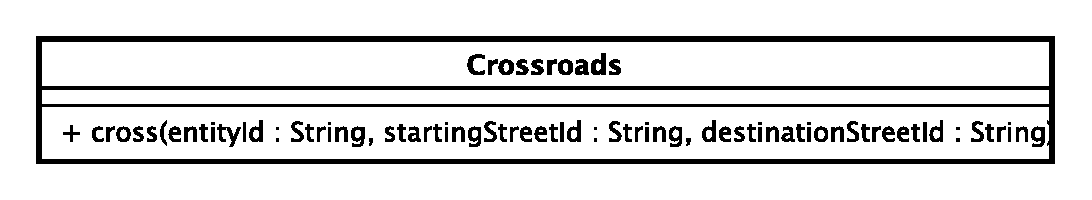
\includegraphics[scale=0.6,keepaspectratio]{diagrams/workspace/application/crossroads.eps}}
\caption{Application::Crossroads}
\end{figure}
\FloatBarrier
A crossroads is a road intersection offers the following operations:
\begin{itemize}
	\item \texttt{cross(entityId : String, startingStreetId : String, destinationStreetId : String)}
	\\Moves an entity from a street to another one
\end{itemize}
%Crossroads’ operations called by entities or roads.
\paragraph{Remarks}
\ \\A crossroads internally encapsulates the logic allows the entities to proceed neatly, i.e. way rules.
%%%%%%%%%%%%%%%%%%%%%%%%%%%%%%%%%
%% CONCURRENCY
%%%%%%%%%%%%%%%%%%%%%%%%%%%%%%%%

\subsubsection{Solution to Concurrency Problems}

Our solution addresses the problems we pointed out in section
\ref{sec:pa-concurrency}. Therefore here we are providing answers to the
questions we made ourselves at the beginning of the development.

\paragraph{How can we recognize that a situation is suitable to present
concurrency?}
There are several active entities in our application: pedestrians, cars, bikes
and buses. They act because of their own initiative, so they are likely to be
considered as active tasks.

Moreover, their actions cause side-effects to reactive entities like roads.
Consequently, our application needs to embody concurrency, i.e., potential
parallelism.

\paragraph{How concurrent accesses will be managed? Will it make sense to
discern side-effect accesses (procedures) from read-only accesses
(\textit{functions})?}
Concurrent accesses will be managed by means of \textit{Protected Objects},
i.e. resources that can be accessed in concurrent read
\textbf{or} mutual exclusive write mode.

It indeed makes sense to have the mentioned separation.
It may be useful to modify roads' status when vehicles travel through them.
Furthermore it might be useful to get information from them
when someone asks for it without causing side-effects.

\paragraph{Which entities have to be active?}
In light of active entities undertake spontaneous actions, in our context they
are:
\begin{itemize}
  \item Moving entities, which move around the city according to their own will;
  \item Semaphores, which autonomously change their color by the time elapses.
\end{itemize}

\paragraph{Which entities have to be reactive?}
Roads (with all their parts) and crossroads should be reactive entities:
\begin{itemize}
  \item A road is used to travel towards a destination and it takes actions
    only when it is trod.
    However, the state of a road is composed of the states of the reactive
    sub-entities it comprises, e.g., stretches and houses;
  \item A crossroads coordinates the traffic at road intersections exclusively
    whenever a moving entity requires to cross it.
\end{itemize}

\paragraph{Which entities have to be passive?}
Passive entities are stateless. Therefore, road signs fit perfectly in this
definition, since they represent immutable information that is read by road
users.

\paragraph{Should we use any formal technique to proof the correctness
of the system properties relating to concurrence?}
We will strive to motivate the correctness of our application but we
deliberately do not choose any specific technique.

\paragraph{Do we have the possibility to incur a non-valid state?
If so, how do we handle the problem?}
The application will be designed to avoid non-valid states. However, if the
system recognizes it is in a non-valid state, it resumes the execution from the
last valid snapshot.
% resumes: see https://www.cs.york.ac.uk/rts/books/RTSbookThirdEdition/chap6.pdf

\paragraph{How can we avoid possible starvation scenarios?}
The application will be designed to overcome starvation or deadlock scenarios.
In fact, active entities do not hold resources.

%%%%%%%%%%%%%%%%%%%%%%%%%%%%%%%%
%% APPLICATION
%%%%%%%%%%%%%%%%%%%%%%%%%%%%%%%%

\subsubsection{Solution to Application Problems}

In section \ref{sec:pa-app-problems} some problems inherently related to the
application domain are explained, and our solution design is thought to solve
them.

\paragraph{Pedestrian Deadlock}
This problem will be avoided ``by design'' by organizing sidewalks in
\textit{lanes}. Though sidewalks in real world usually do not have lanes (apart
from seldom exceptions), we employ the concept of a \textit{logic} lane, i.e.
an abstraction that allows us to coordinate opposite flows of pedestrians in an
agile way.

Since pedestrians proceeding in opposite directions will not compete to enter
the same sidewalk stretch, there can not be any pedestrian deadlock.

\paragraph{Rear-end Collisions}
If the next road stretch of a moving entity route is already taken, the entity
will wait for the stretch to become free before moving on.

\paragraph{Stretch Parallelism}
One road stretch (e.g., a sidewalk stetch) may contain more than one entity of
the same type (e.g., pedestrians) at a time.
Parallelism is achieved by using a system of worker threads thanks to which
more than one active entity can potentially act in parallel in a district.

\paragraph{Yield rules}
The logic to manage yield rules will be encapsulated in crossroads, which has
to ensure the respect of the street code.

\paragraph{Booking a park spot}
A traveller which is going out of a building with a vehicle will try to book
beforehand a spot in the destination building garage, so that when she'll
arrives at destination she will find room to park her vehicle.

Even if this may not seem a concurrency problem at first glance, it is indeed:
two travellers may be leaving from each other's destination, and try to book a
spot in the garages they are leaving.
Therefore, if they both retain a lock on the garage to hold the vehicle they
are coming out with, they are exposed to a deadlock hazard.

We address this issue by making the garage implementation thread-safe, namely
having it be composed of three protected objects:

\begin{itemize}
  \item \textbf{Parked vehicles:} vehicles which are parked in the garage
    without anyone onboard
  \item \textbf{Leaving vehicles:} vehicles which are currently exiting the
    garage
  \item \textbf{Pending vehicles:} vehicles which are not yet arrived in the
    garage
\end{itemize}

Thanks to this division, we are able to avoid holding a lock on the garage
object and access its state concurrently without blocking inside the critical
regions.

%%%%%%%%%%%%%%%%%%%%%%%%%%%%%%%%
%% TIME
%%%%%%%%%%%%%%%%%%%%%%%%%%%%%%%%

\subsubsection{Solution to Time Problems}

In section \ref{sec:pa-time-problems} we point out some questions we made
ourselves about time management in our simulations; hereafter we provide
answers on how we designed the flow of time in our system.

\paragraph{How can we simulate road users proceeding (regarding to travelling
  speed)?}
Our system will be comprehensive of a scheduler, which executes actions
according to an internal agenda.
This agenda is a priority queue in which each entry is matched to a specific
logic instant in time, during which a list of actions has to be executed. This
means active entities will conform to a common interface through which the
scheduler can make them run.

When all the actions for a specific time instant will be executed, the
scheduler will notify other nodes and will wait for a signal (called
\textbf{tick}) to start processing the next entry of its agenda.

%TODO: A cool figure which depicts a scheduler's agenda sample

We will make some speed ranges correspond to a given deferral, so that
travellers with different speeds will take more time to tread stretches with
the same length. For example, a pedestrian might take $25$ logical instants to
move from the beginning to the end of a stretch, whereas a car could take only
$2$ instants to travel the same distance.

We made this choice so that, in the case of a simulation running on several
nodes, our system is far less susceptible to time drift.

\paragraph{How can we simulate crossroads (regarding to road users' arrivals
  time)?}
Crossroads logic will be managed by means of an Ada Protected Object. By
carefully handling concurrent accesses to these objects, we aim to provide the
exact semantic for intersections between roads.

\paragraph{How long do people stay in facilities for? How much precise do these
  intervals have to be?}
Time spent in facilities is decided arbitrarily as a configuration parameter.
These time periods will have the best accuracy provided by the resolution
chosen for the scheduler.

\paragraph{How are semaphores going to be able to synchronize? Which of them
  decide how much time do they have to wait for?}
Semaphores will be active entities, and therefore their actions will be
periodically scheduled.

The period of a semaphore will be a configuration parameter.

\paragraph{When is it suitable to use logical clocks instead of local system
  clock?}
As for our simulations, logical time will be used for nearly everything so that
our application will not suffer to drift caused by computation on different
nodes.

However, we will seldom rely on wall clock time for specific operations, like
request timeouts for RPCs.



% Artificial Intelligence subsection
\subsection{Artificial Intelligence (AI)}

Our AI offers three path finding algorithms:
\begin{itemize}
  \item Greedy Search;
  \item Uniform Cost Search;
  \item A* Search.
\end{itemize}

The first one is incomplete and not optimal because of the local search which looks only one step ahead (visiting
only the neighbors). The last two algorithm are both complete and optimal under certain assumptions. They have been defined
to guarantee our agents to always find the best possible path with the minimum number of visited nodes in the search graph.

To guarantee completeness we need to assume that each graph is a strongly
connected component. Basically, it means that there are no isolated
components. Thus, the agent knows there will always be at least a path between
the source and the destination of its plan. % its or her

Furthermore, our AI considers not grid based maps: which means some common
heuristics are not applicabile a priori (e.g. Manhattan distance, euclidean
distance). Also, since grid-based maps are a subset of all possible maps, we
can say that our AI is independent on the map toopology.

To solve the path finding problem we reason about the specific domain and its
abstractions in terms of infrastructure building blocks and travellers. We
found an admissibile and consistent heuristic for A* and in general other
informed algorithms. To concretely guarantee the assumptions hold for all the
graph configurations we apply the Tarjan algorithm.

Tarjan automatically validates our graphs at build time by ensuring that there
is only one strong connected component for each graph, otherwise it reports
an error and shows the isolated component.
Finally, the AI is agent-independent, which means we can use it to calculate
the path of different kinds of agents: bicycles which move on bicycle lanes,
pedestrians who move on sidewalks and motor vehicles which move on roads.


